% =====================================================================
% Capítulo: Pruebas y Resultados
% =====================================================================

\chapter{Pruebas y Resultados}\label{chap:resultados}

Este capítulo evalúa AST-CC en dos etapas. La primera usa datos sintéticos, en los
que la estructura verdadera es conocida, para comprobar que el método controla los
refinamientos espurios, que encuentra los patrones locales cuando existen, que
repara una partición base que agrupa mal sin inventar estructura y que lo hace
mejor que una rejilla global más fina. La segunda aplica el método a la partición
de ST-CC sobre los datos de taxis de Manhattan, describe los cortes que encuentra,
fija el umbral $\delta$ con datos que el árbol no vio, lo compara con ST-CC y con
rejillas globales optimizadas, mide la estabilidad y la replicación de sus cortes e
interpreta los patrones que revelan. El capítulo termina con las limitaciones de
estos resultados.

% ---------------------------------------------------------------------
\section{Datos y configuración experimental}\label{sec:res-datos}

Los experimentos con datos reales usan los mismos registros que el caso de estudio
de ST-CC descrito en la Sección~\ref{sec:stcc}, es decir, las bajadas de los taxis
amarillos y verdes en las 66 zonas de Manhattan durante noviembre de 2017,
agregadas en 12 intervalos de dos horas y separadas en un periodo laborable de
$D = 12$ días, que son los martes a jueves del mes salvo el Día de Acción de
Gracias y la víspera, y un periodo feriado de $D = 9$ días, que son los sábados,
los domingos y el Día de Acción de Gracias. A diferencia de
\citet{Liu2021}, que trabajan con el volumen promedio por día, AST-CC trabaja con la
matriz de conteos, que es la suma de los días del periodo, porque las pruebas de
hipótesis necesitan la escala real de los datos (Sección~\ref{sec:escala}). Esa
matriz reúne $N = 3\,602\,851$ viajes en el periodo laborable y $N = 2\,389\,795$
en el feriado, y cada día se conserva además como una matriz propia, que es la
unidad que remuestrea el \emph{bootstrap} de días. Para evaluar el método fuera de
la muestra se usan también los otros once meses de 2017, con la misma regla de
selección de días, es decir, los martes a jueves para el periodo laborable y los
sábados y domingos para el feriado, excluyendo los días atípicos, que son el Año
Nuevo, el 4 de julio, las nevadas del 9 de febrero y del 14 y 15 de marzo, y las
fiestas de fin de año del 21 al 31 de diciembre. Resultan 134 días laborables con
$40\,024\,248$ viajes y 92 días de fin de semana con $25\,642\,581$ viajes, que el
árbol nunca ve durante el ajuste y que solo se usan para medir si los cortes
encontrados en noviembre se sostienen en el resto del año. La
Tabla~\ref{tab:res-datos} resume ambos conjuntos.

\begin{table}[t]
\centering
\small
\begin{tabular}{lrrrrc}
\toprule
 & \multicolumn{2}{c}{Noviembre de 2017} & \multicolumn{2}{c}{Resto de 2017} & \\
\cmidrule(lr){2-3}\cmidrule(lr){4-5}
Periodo & Días & Viajes & Días & Viajes & $K_R \times K_T$ \\
\midrule
Laborable & 12 & 3\,602\,851 & 134 & 40\,024\,248 & $8 \times 4$ \\
Feriado   &  9 & 2\,389\,795 &  92 & 25\,642\,581 & $6 \times 4$ \\
\bottomrule
\end{tabular}
\caption{Datos de los experimentos. Noviembre se usa para ajustar el árbol y el
resto de 2017 solo para evaluarlo. La última columna es la resolución de la
partición base de ST-CC.}
\label{tab:res-datos}
\end{table}

{\emergencystretch=2em
La partición base que refina AST-CC es la de ST-CC tal como se obtiene al
reproducir el método con el paquete \texttt{clustering-geodata-cubes}
\citep{Nattino2022}, con los valores de \citet{Liu2021}, $K_R \times K_T = 8 \times 4$ en el periodo laborable y
$6 \times 4$ en el feriado, es decir, 32 y 24 bloques base. Se parte de esa
partición y no de una optimizada por esta tesis para que toda diferencia entre
ST-CC y AST-CC se deba únicamente al árbol, que es la pregunta que plantean los
objetivos. Como esa implementación corresponde a la base C2
(Sección~\ref{sec:stcc-base}), sus bloques agrupan regiones e intervalos por su
volumen y no por la forma de su perfil, de modo que dentro de ellos queda una
interacción local considerable. Medido con el término (iii) de la
Proposición~\ref{prop:descomposicion}, ese residuo es de $25\,703$ nats en el
periodo laborable y de $43\,011$ en el feriado, que es la cantidad que el árbol
puede explicar. Las particiones obtenidas con BBAC$_I$ en la base C5 y la rejilla
del mismo tamaño optimizada para el modelo de las hojas se usan solo como análisis
de sensibilidad (Sección~\ref{sec:res-sensibilidad}).\par}

Los parámetros de AST-CC son los de la Tabla~\ref{tab:prop-parametros}, con un
nivel global $\alpha = 0.05$, la nula del \emph{bootstrap} de días con la
fluctuación corregida, al menos $B_{\min} = 199$ réplicas y a lo sumo
$B_{\max} = 20\,000$ por bloque, resolución $c = 2$ respecto de $\alpha_B$, parada
secuencial inspirada en \citet{Besag1991} con $h = 10$, $N_{\min} = 500$ viajes y
profundidad máxima $d_{\max} = 6$. Entre dos cortes admisibles, es decir,
significativos y con ganancia corregida de al menos $\delta$, se aplica el de mayor
$z$. El umbral $\delta$ se usa en dos niveles con papeles distintos. El árbol
completo usa $\delta = 0.00025$ nats por viaje, valor a partir del cual el árbol
deja de cambiar, y es el modelo que se compara con ST-CC y con las rejillas
globales. El árbol resumido usa $\delta = 0.005$ en el periodo laborable y
$\delta = 0.02$ en el feriado, que dejan del orden de 10 a 15 cortes, y es el que
se interpreta y se dibuja. La Sección~\ref{sec:res-delta} muestra que los datos no
permiten fijar un único $\delta$, porque todos los cortes de la rejilla se
replican fuera de la muestra, y por eso $\delta$ se trata como un umbral de
resolución y no como un parámetro estadístico. Todas las ejecuciones usan
semillas fijas, y el código y los resultados están en el repositorio de la tesis.

% ---------------------------------------------------------------------
\section{Calibración y potencia con datos sintéticos}\label{sec:res-sinteticos}

Esta sección responde dos preguntas que el Capítulo~\ref{chap:propuesta} dejó
abiertas. La primera es si el método completo controla los refinamientos espurios
cuando los datos no comparten el mecanismo del \emph{bootstrap} de días, ya que la
calibración de la Tabla~\ref{tab:prop-calibracion} usó datos semirreales generados
con ese mismo mecanismo, lo que podía favorecerlo. La segunda es si ese control se
mantiene cuando la partición base se estima con los mismos datos que luego se
prueban, que es la situación real y la que la Sección~\ref{sec:prop-multiplicidad}
no cubre con una garantía formal. A ellas se suma la potencia, es decir, la
capacidad de encontrar un patrón local cuando existe y de separarlo con el corte
correcto.

\subsection{Diseño de los datos sintéticos}

Los datos sintéticos reproducen el tamaño del periodo laborable, con una matriz de
$66 \times 12$, un tablero base de $8 \times 4$ bloques, $D = 12$ días y alrededor
de tres millones de viajes. La media de cada celda es el producto de un efecto de
fila, un efecto de columna y un nivel propio del bloque, con efectos de fila y de
columna desiguales como los de la movilidad real, de modo que dentro de cada bloque
sin patrón se cumple exactamente la independencia y cualquier corte en él es un
falso descubrimiento. Cada día se genera multiplicando esa media por un efecto
común a todo el día, por efectos propios de cada día y región y de cada día e
intervalo, todos lognormales de media uno, y por un ruido gamma de celda, y
tomando después un conteo de Poisson. Este mecanismo es distinto del
\emph{bootstrap}, que remuestrea días observados, y produce desviaciones
correlacionadas entre celdas parecidas a las de los datos reales
(Sección~\ref{sec:prop-sobredispersion}). Se usan tres escenarios de
variabilidad entre días. El escenario Poisson no tiene efectos de día ni ruido de
celda. El escenario realista tiene efectos de día de escala 0.03, efectos de día y
región y de día e intervalo de escala 0.07 y ruido gamma de forma 200, con lo que
el cociente entre la varianza y la media de los conteos diarios de cada celda es
de alrededor de 3.1, como la mediana de 3.2 del periodo laborable
(Tabla~\ref{tab:prop-dispersion}). El escenario fuerte usa 0.10, 0.15 y forma
100, con un cociente cercano a 10, que se acerca al del periodo feriado sin
alcanzar su mediana de 17.1. Este cociente no es la dispersión de Pearson de 2.06
y 6.73 que se usa en la Sección~\ref{sec:res-comparacion}, que se mide después de
quitar los efectos de día y región y de día e intervalo. Los patrones se plantan multiplicando por un
factor $f$ la media de la mitad de las filas de un bloque en la mitad de sus
columnas, y su tamaño se resume con la información mutua poblacional del bloque,
$I_{\mathrm{pob}}$, que es la cantidad que el árbol intenta detectar y que se
compara directamente con $\delta$.

\subsection{Calibración}

La Tabla~\ref{tab:res-calibracion} muestra la tasa de error por familia, medida
como la proporción de 200 réplicas sin patrones en las que el árbol hace al menos un
corte. Con $\delta = 0$, que es el caso más exigente porque solo decide la prueba,
la nula del \emph{bootstrap} mantiene el FWER por debajo del nivel nominal en los
tres escenarios, con 0.000, 0.005 y 0.030, mientras que la nula de Poisson solo es
válida cuando los datos son realmente de Poisson y fracasa en cuanto hay
variabilidad entre días, con un FWER de 1 y entre 13 y 26 cortes espurios por
réplica. Con $\delta = 0.005$ ninguna de las dos nulas produce cortes, pero eso no
rehabilita a la de Poisson, porque es el umbral el que oculta su falla. El árbol
completo trabaja con un $\delta$ veinte veces menor, que ya no la oculta, de modo
que con ese umbral el control de los cortes espurios depende de que la prueba sea
válida por sí misma. Como un $\delta$ positivo solo puede eliminar cortes, el
FWER con el $\delta$ del árbol completo queda acotado por el que se obtiene con
$\delta = 0$. La última fila responde la segunda pregunta. Cuando la partición
base se estima con BBAC$_I$ en la base C5 a partir de los mismos datos, el FWER es
0.020, dentro del nivel nominal, de modo que la selección de la partición no
infla los refinamientos espurios en la práctica, aunque la garantía de la
Sección~\ref{sec:prop-multiplicidad} sea solo aproximada. Esta fila usa la base C5
porque es la que corresponde al modelo del generador y recupera sus bloques, con lo
que dentro de ellos se cumple la nula. Lo que ocurre con una base que no
recupera los bloques, como la de ST-CC, no es un problema de calibración sino de
reparación de la base, y se estudia en la Sección~\ref{sec:res-reparacion}.

\begin{table}[t]
\centering
\small
\begin{tabular}{@{}lllccc@{}}
\toprule
 & & & \multicolumn{2}{c}{$\delta = 0$} & $\delta = 0.005$ \\
\cmidrule(lr){4-5}\cmidrule(l){6-6}
Escenario & Partición base & Nula & FWER & Cortes por réplica & FWER \\
\midrule
Poisson  & verdadera & Poisson             & 0.040 & 0.04  & 0.000 \\
Poisson  & verdadera & \emph{bootstrap}    & 0.000 & 0.00  & 0.000 \\
Realista & verdadera & Poisson             & 1.000 & 13.23 & 0.000 \\
Realista & verdadera & \emph{bootstrap}    & 0.005 & 0.01  & 0.000 \\
Fuerte   & verdadera & Poisson             & 1.000 & 26.21 & 0.000 \\
Fuerte   & verdadera & \emph{bootstrap}    & 0.030 & 0.03  & 0.000 \\
Realista & BBAC$_I$ C5 & \emph{bootstrap}  & 0.020 & 0.02  & 0.020 \\
\bottomrule
\end{tabular}
\caption{Tasa de error por familia (FWER) de AST-CC sobre 200 réplicas sintéticas
sin patrones locales, al nivel $\alpha = 0.05$. El error de Monte Carlo es de
aproximadamente 0.015.}
\label{tab:res-calibracion}
\end{table}

\subsection{Potencia y recuperación del patrón}

La Tabla~\ref{tab:res-potencia} muestra, en el escenario realista con la
partición verdadera, la proporción de patrones cuyo bloque se refina, para cinco
factores, para los dos niveles de $\delta$ de la Sección~\ref{sec:res-datos} y,
como referencia, para $\delta = 0$. La
detección crece con el tamaño del efecto, de 0.54 con $I_{\mathrm{pob}} = 0.0007$
a 0.94 con 0.0019 y a prácticamente 1 desde 0.0035, y cuando el bloque se refina el
primer corte separa casi exactamente las filas activadas, con un índice de Rand
ajustado entre 0.94 y 1 desde el factor 1.2. El $\delta$ del árbol completo no cuesta
potencia frente a $\delta = 0$, porque solo descarta efectos menores que su propia
escala, que tampoco se detectan sin él. El $\delta$ del árbol resumido, en cambio,
actúa como un umbral sobre el tamaño del efecto, tal como se pretende, ya que
detecta el 90\,\% de los patrones con $I_{\mathrm{pob}} = 0.0092$, por encima de
0.005, y solo el 11\,\% de los de 0.0035, por debajo. En ningún caso se refinó
un bloque sin patrón en más del 2\,\% de las réplicas.

\begin{table}[t]
\centering
\small
\begin{tabular}{@{}ccccccc@{}}
\toprule
 & & \multicolumn{3}{c}{Proporción detectada} & & \\
\cmidrule(lr){3-5}
Factor $f$ & $I_{\mathrm{pob}}$ & $\delta = 0$ & $\delta = 0.00025$ & $\delta = 0.005$ & ARI & Falsos \\
\midrule
1.1  & 0.0002 & 0.06 & 0.04 & 0.00 & 0.81 & 0.02 \\
1.2  & 0.0007 & 0.54 & 0.54 & 0.00 & 0.94 & 0.00 \\
1.35 & 0.0019 & 0.94 & 0.94 & 0.00 & 0.99 & 0.02 \\
1.5  & 0.0035 & 0.98 & 0.98 & 0.11 & 0.98 & 0.00 \\
2.0  & 0.0092 & 1.00 & 1.00 & 0.90 & 1.00 & 0.00 \\
\bottomrule
\end{tabular}
\caption{Potencia de AST-CC en el escenario realista, con la partición base
verdadera y dos patrones por réplica (60 réplicas). El ARI es el índice de Rand
ajustado entre el primer corte y las filas activadas, promediado sobre los patrones
detectados con $\delta = 0.00025$, que con factor 1.1 son muy pocos, y la última columna es la proporción de
réplicas con algún corte en un bloque sin patrón con ese mismo $\delta$.}
\label{tab:res-potencia}
\end{table}

El patrón anterior es el más sencillo, por lo que se evaluaron otros tres que ponen
a prueba partes distintas del método, junto con el mismo patrón sobre una partición
base estimada (Tabla~\ref{tab:res-patrones}). El patrón en tablero activa unas
filas en unas columnas y otras filas en las demás, de modo que los totales del
bloque apenas cambian. Aun así se detecta en el 98\,\% de las réplicas desde el
factor 1.25, lo que confirma que la prueba ómnibus lo ve y que un corte de filas lo
separa. El patrón anidado contiene dos grupos de filas con perfiles distintos en el
mismo bloque y exige dos cortes sucesivos. Con factor 1.5 el árbol llega a
profundidad 2 en todas las réplicas, con un índice de Rand ajustado de 0.94. El
patrón que cruza activa un grupo de filas en columnas de dos grupos de intervalos,
por lo que queda repartido entre dos bloques base, y el árbol lo refina en ambos.
Por último, cuando la base se estima con BBAC$_I$, la proporción refinada baja a
0.72 y 0.85 para los factores 1.25 y 1.5, pero no porque el árbol pierda el patrón.
En el 5 y el 15\,\% de las réplicas la propia partición estimada ya lo aísla en
un grupo propio, lo que deja al árbol sin nada que refinar, y por eso el índice de
Rand ajustado llega a 1 con factor 1.5.

\begin{table}[t]
\centering
\small
\begin{tabular}{@{}lcccccc@{}}
\toprule
 & \multicolumn{3}{c}{$f = 1.25$} & \multicolumn{3}{c}{$f = 1.5$} \\
\cmidrule(lr){2-4}\cmidrule(l){5-7}
Patrón & Refina & ARI & Prof. & Refina & ARI & Prof. \\
\midrule
Simple                       & 0.77 & 0.74 & 0.8 & 1.00 & 0.99 & 1.0 \\
Simple, base de BBAC$_I$     & 0.72 & 0.77 & 0.7 & 0.85 & 1.00 & 0.9 \\
Tablero                      & 0.98 & 0.98 & 1.0 & 1.00 & 1.00 & 1.0 \\
Anidado                      & 0.97 & 0.71 & 1.5 & 1.00 & 0.94 & 2.0 \\
Cruzado entre bloques        & 0.90 & 0.72 & 0.9 & 1.00 & 0.96 & 1.0 \\
\bottomrule
\end{tabular}
\caption{Recuperación de distintos tipos de patrón con $\delta = 0.00025$ en el
escenario realista (60 réplicas). Refina es la proporción de réplicas en que se
refina algún bloque con el patrón, ARI es el acuerdo entre las hojas y los grupos
verdaderos, promediado sobre todas las réplicas, y Prof. es la profundidad media
de las hojas en los bloques con patrón. La proporción de réplicas con algún corte
espurio no superó 0.03 en ningún caso. A diferencia de la
Tabla~\ref{tab:res-potencia}, que cuenta patrones detectados y promedia el ARI
solo sobre ellos, aquí se cuentan réplicas y el ARI se promedia sobre todas, por
lo que las cifras del patrón simple no coinciden exactamente entre ambas tablas.}
\label{tab:res-patrones}
\end{table}

% ---------------------------------------------------------------------
\section{Reparación de una partición base agrupada por volumen}\label{sec:res-reparacion}

La calibración de la sección anterior supone que la partición base recupera los
bloques verdaderos, de modo que dentro de ellos se cumple la independencia y todo
corte es un error. Con los datos reales no ocurre así. La partición de ST-CC que
refina AST-CC corresponde a la base C2 (Sección~\ref{sec:stcc-base}), que agrupa
regiones e intervalos por su volumen y no por la forma de su perfil, de manera que
puede reunir en un mismo bloque regiones que se llenan a horas distintas. Dentro
de esos bloques la independencia no se cumple y los cortes del árbol no son
errores sino correcciones de la base. Lo que debe comprobarse entonces es que esas
correcciones recuperan la estructura verdadera de los datos y no inventan una
distinta. Para ello se generaron 40 réplicas de cada uno de los escenarios
realista y fuerte de la Sección~\ref{sec:res-sinteticos}, sin patrones locales,
de modo que la verdad es una rejilla de $8 \times 4$ bloques con independencia
dentro de cada uno, y se ajustó AST-CC sobre tres particiones base, la verdadera,
la estimada con BBAC$_I$ en la base C5 y la estimada con BBAC$_I$ en la base C2,
que reproduce el esquema de ST-CC. La calidad de cada ajuste se mide con la
divergencia de Kullback--Leibler entre las proporciones verdaderas de las celdas
y las ajustadas, en milésimas de nat por viaje. Esa divergencia no llega a cero
ni siquiera con la partición verdadera, porque los parámetros de cada bloque se
estiman con datos finitos, y su valor con la partición verdadera es por eso el
mínimo alcanzable. Como medida complementaria se usa la pureza, que es la
fracción de la masa verdadera de cada hoja que cae en su bloque verdadero
mayoritario, ponderada por masa, y que vale 1 cuando ninguna hoja mezcla bloques
verdaderos.

\begin{table}[t]
\centering
\small
\begin{tabular}{@{}lccccccccc@{}}
\toprule
 & & & \multicolumn{2}{c}{Sin cortes} & \multicolumn{3}{c}{$\delta = 0.00025$} & \multicolumn{2}{c}{$\delta = 0.005$} \\
\cmidrule(lr){4-5}\cmidrule(lr){6-8}\cmidrule(l){9-10}
Partición base & \multicolumn{2}{c}{ARI} & KL & Pureza & Cortes & KL & Pureza & Cortes & KL \\
\midrule
\multicolumn{10}{@{}l}{Escenario realista} \\
Verdadera         & 1.00 & 1.00 & 0.51  & 1.000 & 0.0  & 0.51 & 1.000 & 0.0  & 0.51 \\
BBAC$_I$ C5       & 0.94 & 0.99 & 0.51  & 0.971 & 0.0  & 0.51 & 0.971 & 0.0  & 0.51 \\
BBAC$_I$ C2       & 0.10 & 0.36 & 21.49 & 0.457 & 30.5 & 0.59 & 0.588 & 22.6 & 1.06 \\
\midrule
\multicolumn{10}{@{}l}{Escenario fuerte} \\
Verdadera         & 1.00 & 1.00 & 2.09  & 1.000 & 0.1  & 2.10 & 1.000 & 0.0  & 2.09 \\
BBAC$_I$ C5       & 0.92 & 1.00 & 2.10  & 0.968 & 0.1  & 2.10 & 0.968 & 0.0  & 2.10 \\
BBAC$_I$ C2       & 0.12 & 0.38 & 21.92 & 0.470 & 29.7 & 2.26 & 0.597 & 22.6 & 2.71 \\
\bottomrule
\end{tabular}
\caption{AST-CC sobre datos sintéticos sin patrones locales con tres particiones
base (40 réplicas por escenario). Las dos columnas de ARI son el acuerdo de la
partición base con la verdadera en filas y en columnas. KL es la divergencia entre
las proporciones verdaderas y las ajustadas, en milésimas de nat por viaje, y la
pureza es la fracción de la masa de cada hoja que cae en su bloque verdadero
mayoritario.}
\label{tab:res-reparacion}
\end{table}

La Tabla~\ref{tab:res-reparacion} resume los resultados. Con la partición
verdadera y con la de la base C5, que recupera los bloques con un índice de Rand
ajustado de al menos 0.92, el árbol prácticamente no corta, lo que repite la
calibración de la sección anterior. La partición de la base C2, en cambio, apenas
se parece a la verdadera, con un índice de Rand ajustado de 0.10 en las filas, y
sin cortes su ajuste es más de cuarenta veces peor que el mínimo alcanzable en el
escenario realista, con 21.49 frente a 0.51. Sobre esa base el árbol hace unos 30
cortes por réplica y lleva la divergencia a 0.59, con lo que elimina el 99.6\,\%
del exceso de la base sobre el mínimo, y en el escenario fuerte elimina el
99.1\,\%. Incluso el árbol resumido, con $\delta = 0.005$ y unos 23 cortes,
elimina el 97\,\% de ese exceso en ambos escenarios. El árbol, por tanto, no
inventa estructura, porque sobre una base correcta no corta, y cuando la base
agrupa mal reconstruye casi por completo la distribución verdadera.

La pureza matiza este resultado. Sobre la base C2 sube de 0.46 a 0.59, de modo que
las hojas siguen mezclando bloques verdaderos aunque el ajuste sea casi perfecto.
Esto se debe a que el modelo de las hojas solo exige independencia dentro de cada
una, y una hoja que reúne filas de bloques verdaderos distintos la cumple igual
si en sus intervalos esas filas tienen perfiles proporcionales, lo que ocurre
siempre, por ejemplo, en una hoja de un solo intervalo. El árbol encuentra así
una partición que describe bien los datos, pero que no coincide con la que los
generó, y para describir la misma distribución puede necesitar más hojas que la
rejilla verdadera. De aquí se sigue cómo deben leerse los cortes del árbol sobre
la partición de ST-CC en los datos reales. Cada corte indica con fundamento que
ST-CC reunió en un mismo bloque regiones o intervalos con perfiles distintos y
dónde ocurre, pero sus hojas no deben interpretarse como las unidades naturales de
la ciudad, sino como la corrección más sencilla que el árbol encontró para cada
bloque.

% ---------------------------------------------------------------------
\section{AST-CC frente a rejillas globales con verdad conocida}\label{sec:res-rejillas-sinteticos}

La alternativa más directa a refinar localmente es aumentar la resolución de la
rejilla global, es decir, usar más grupos de regiones o de intervalos en toda la
matriz. Si una rejilla más fina con el mismo número de parámetros recuperara lo
mismo que el árbol, AST-CC no aportaría nada. Con los datos reales esta comparación
solo puede hacerse con el ajuste o con días no usados (Sección~\ref{sec:res-comparacion}),
mientras que con datos sintéticos puede medirse contra la verdad. Para ello se
generaron 100 réplicas del escenario realista con cinco tipos de patrón, el
simple con factores 1.25, 1.5 y 2, y el de tablero y el anidado con factor 1.5. En
cada réplica la partición base de $8 \times 4$ se estimó con BBAC$_I$ en la base
C5, que recupera los bloques del generador, de modo que el árbol solo tiene que
encontrar los patrones y no reparar la base. Cada ajuste se compara con la media
verdadera $\mu$ mediante la divergencia $D_I(\mu \,\|\, \hat O)$, en nats, que mide
la distancia a la estructura que generó los datos y no a otra realización de su
ruido. El rival de AST-CC es la rejilla de menos parámetros entre las que tienen al
menos tantos como el árbol, lo que le da ventaja a la rejilla, y se optimiza
directamente para el modelo de las hojas, de independencia dentro de cada bloque,
que es el modelo C6 de la Sección~\ref{sec:bases},
partiendo de las particiones de BBAC$_I$ en las bases C2 y C5. Como referencia se
incluyen la rejilla del mismo tamaño tomada de BBAC$_I$ sin esa optimización, la
partición base sin cortes y el modelo saturado, que reproduce los datos celda a
celda.

\begin{table}[t]
\centering
\small
\begin{tabular}{@{}lcccccccc@{}}
\toprule
 & Base & \multicolumn{2}{c}{AST-CC} & \multicolumn{3}{c}{Rejilla global} & Saturado & Gana \\
\cmidrule(lr){3-4}\cmidrule(lr){5-7}
Patrón & $D_I$ & $k$ & $D_I$ & $k$ & $D_I$ (C6) & $D_I$ (BBAC$_I$) & $D_I$ & el árbol \\
\midrule
Simple, $f = 1.25$ & 2\,448 & 331 & 2\,181 & 342 & 2\,448 & 2\,337 & 2\,743 & 100\,\% \\
Simple, $f = 1.5$  & 2\,654 & 331 & 1\,945 & 344 & 2\,218 & 2\,493 & 2\,523 & 100\,\% \\
Simple, $f = 2$    & 4\,275 & 331 & 2\,006 & 344 & 2\,268 & 3\,118 & 2\,587 & 100\,\% \\
Tablero, $f = 1.5$ & 3\,875 & 330 & 2\,063 & 342 & 2\,335 & 3\,402 & 2\,656 & 100\,\% \\
Anidado, $f = 1.5$ & 3\,497 & 332 & 2\,099 & 344 & 2\,380 & 3\,020 & 2\,687 & 100\,\% \\
\bottomrule
\end{tabular}
\caption{Distancia a la media verdadera, $D_I(\mu \,\|\, \hat O)$ en nats, de la
partición base sin cortes, de AST-CC con $\delta = 0.00025$, de la rejilla global
de menos parámetros con al menos tantos como el árbol (optimizada para el modelo
C6 y tomada de BBAC$_I$ sin optimizar) y del modelo saturado, como media de 100
réplicas del escenario realista con $k = 328$ parámetros en la base. La última
columna es la proporción de réplicas en que el árbol queda más cerca de la verdad
que la rejilla optimizada.}
\label{tab:res-rejillas-sinteticos}
\end{table}

La Tabla~\ref{tab:res-rejillas-sinteticos} muestra que el árbol queda más cerca de
la verdad que la rejilla global en el 100\,\% de las réplicas de los cinco
escenarios, con una diferencia media de entre 260 y 280 nats, y lo logra con menos
parámetros, porque añade solo dos a cuatro a los 328 de la base, mientras que la
rejilla necesita al menos 342. La razón es que la rejilla tiene que gastar sus
parámetros en toda la matriz para separar un patrón que vive en un solo bloque, y
al aumentar un grupo de regiones o de intervalos parte también los bloques
donde no hay nada que separar. Por eso la rejilla optimizada no mejora a la
base cuando el patrón es débil, con 2\,448 frente a 2\,448 en el escenario simple
con factor 1.25, mientras que el árbol baja a 2\,181. La rejilla tomada de
BBAC$_I$ sin optimizar para el modelo de las hojas es peor que la optimizada en
cuatro de los cinco escenarios, con diferencias de 275 a 1\,067 nats, lo que
muestra que la comparación justa exige optimizar la rejilla con el mismo criterio
con que se evalúa. La excepción es el patrón simple con factor 1.25, en el que la
rejilla de BBAC$_I$ queda más cerca de la verdad, con 2\,337, porque la
optimización minimiza la divergencia con los datos y, cuando el patrón es débil,
gasta sus grupos adicionales en ajustar el ruido. Aun así, el árbol también la
supera, en el 89\,\% de las réplicas. El modelo saturado queda lejos de la verdad en todos los casos porque
reproduce también el ruido de los datos, con distancias de 2\,500 a 2\,700 nats,
peores que las del árbol y en general que las de la rejilla.

Los resultados con $\delta = 0$ son prácticamente idénticos a los de
$\delta = 0.00025$, lo que confirma que el $\delta$ del árbol completo no cuesta
potencia. Como medida complementaria se calculó el índice de Rand ajustado entre
las celdas del patrón plantado y los grupos de cada método dentro del bloque con
patrón, que en el patrón simple es de 0.33 a 0.45 para el árbol y de 0.09 a 0.11
para la rejilla. El árbol no llega a 1 porque separa las filas activadas con un solo
corte de filas y no aísla las celdas activas de las inactivas de esas filas, pero
no necesita hacerlo, porque todas las filas activadas tienen el mismo perfil y el
modelo de independencia de la hoja ya las describe exactamente. Por la misma razón,
en los patrones de tablero y anidado este índice es bajo para todos los métodos,
y la medida que importa es la distancia a la verdad.

% ---------------------------------------------------------------------
\section{AST-CC sobre los datos reales}\label{sec:res-arbol}

La Tabla~\ref{tab:res-arboles} resume los árboles ajustados sobre la partición de
ST-CC en los dos periodos y con los dos niveles de $\delta$. El árbol completo
hace 71 cortes en el periodo laborable y 52 en el feriado, llega a profundidad 5
y 4, y explica el 95.9\,\% y el 90.7\,\% del término (iii) de la
Proposición~\ref{prop:descomposicion}, es decir, de la interacción que la
partición de ST-CC deja dentro de sus bloques. Que el árbol explique casi toda
esa interacción es lo esperable según la Sección~\ref{sec:res-reparacion}, porque
la partición de ST-CC agrupa por volumen y reúne en un mismo bloque regiones e
intervalos con perfiles distintos. El árbol resumido conserva solo los cortes
cuya ganancia corregida supera $0.005$ nats por viaje en el periodo laborable y
$0.02$ en el feriado, con 13 y 15 cortes, y aun así explica el 64.8\,\% y el
54.0\,\% de esa interacción, de modo que unos pocos cortes concentran la mayor
parte de lo que ST-CC no captura. La mayoría de los cortes son de filas, es
decir, separan regiones dentro de un mismo grupo de intervalos, aunque en el árbol
completo del periodo laborable casi un tercio son de columnas, de modo que a esa
resolución también la agrupación temporal de ST-CC resulta gruesa. Los tipos de
hoja son los de la Sección~\ref{sec:prop-parada}. Las hojas inalcanzables son
bloques cuyo nivel $\alpha_B$, que se reparte en proporción a su número de viajes,
queda por debajo del menor p-valor que permiten 20\,000 réplicas, por lo que no
pueden probarse, y en estos datos son los bloques del grupo de regiones de menor
volumen con apenas unos miles de viajes en todo el mes. Un bloque de ese mismo
grupo con algo más de masa sí puede probarse, como el del corte de mayor ganancia
del periodo feriado. Las hojas triviales tienen una sola fila o un solo intervalo,
por lo que no admiten interacción, y son casi siempre bloques de un solo intervalo, como el de 06--08 en el periodo
laborable, que ST-CC dejó aislado y que no admiten interacción.

\begin{table}[t]
\centering
\small
\begin{tabular}{@{}llcccccc@{}}
\toprule
Periodo & Árbol & $\delta$ & Hojas & Cortes (f / c / conj.) & Prof. & (iii) expl. & Inalc. \\
\midrule
Laborable & completo & 0.00025 & 105 & 47 / 23 / 1 & 5 & 95.9\,\% & 4 \\
Laborable & resumido & 0.005   & 45  & 11 / 2 / 0  & 2 & 64.8\,\% & 3 \\
Feriado   & completo & 0.00025 & 78  & 48 / 3 / 1  & 4 & 90.7\,\% & 7 \\
Feriado   & resumido & 0.02    & 39  & 12 / 3 / 0  & 2 & 54.0\,\% & 6 \\
\bottomrule
\end{tabular}
\caption{Árboles de AST-CC sobre la partición de ST-CC, con 32 bloques base en
el periodo laborable y 24 en el feriado. Los cortes se separan en cortes de filas,
de columnas y conjuntos, (iii) expl. es la fracción de la interacción local de
ST-CC que explican los cortes del árbol e Inalc. el número de hojas inalcanzables.}
\label{tab:res-arboles}
\end{table}

\subsection{Árbol resumido del periodo laborable}

La Figura~\ref{fig:res-teselada} muestra la matriz teselada del árbol resumido y
la Figura~\ref{fig:res-refinados} sitúa en el mapa las regiones que separa cada
corte. El patrón dominante aparece en el grupo de intervalos diurnos, de 08--10 a
16--18, donde ocho de los trece cortes separan regiones que reciben sus llegadas
temprano de regiones que las reciben por la tarde. El corte de mayor ganancia, con
$\tilde g = 0.027$, parte un bloque de trece regiones de volumen bajo en dos
grupos. En Alphabet City, Bloomingdale, Hamilton Heights, Stuy Town, Two Bridges y
Washington Heights North el 29.2\,\% de las llegadas diurnas ocurre entre las 16 y
las 18 horas, mientras que en el Financial District South, el World Trade Center,
el Seaport, Chinatown, Hudson Square, Manhattanville y Washington Heights South
esa fracción es del 13.8\,\% y el máximo está entre las 8 y las 10, con el
28.2\,\%. Lo mismo ocurre entre las zonas de mayor volumen. En Midtown Center y
Midtown East el 28.9\,\% de las llegadas diurnas ocurre entre las 8 y las 10,
frente al 18.3\,\% en el Upper East Side. Es la huella del desplazamiento al
trabajo, en la que las zonas de oficinas reciben a los viajeros por la mañana y
las residenciales al regreso, y ST-CC las había reunido porque tienen volúmenes
diarios parecidos, de 7\,752 y 8\,706 llegadas por región y día en el caso de
Midtown y el Upper East Side. Un corte del mismo tipo separa Midtown North, Murray
Hill, Times Square y Union Square de Lincoln Square East y Penn Station, y la
diferencia entre esos dos grupos se mantiene en el resto de 2017, pero el árbol
casi nunca llega a ese corte cuando la partición de partida cambia, porque sus
hojas tienen soportes de 0 y 0.35 (Sección~\ref{sec:res-estabilidad}), y por eso
no se cuenta entre los hallazgos.

\begin{figure}[t]
\centering
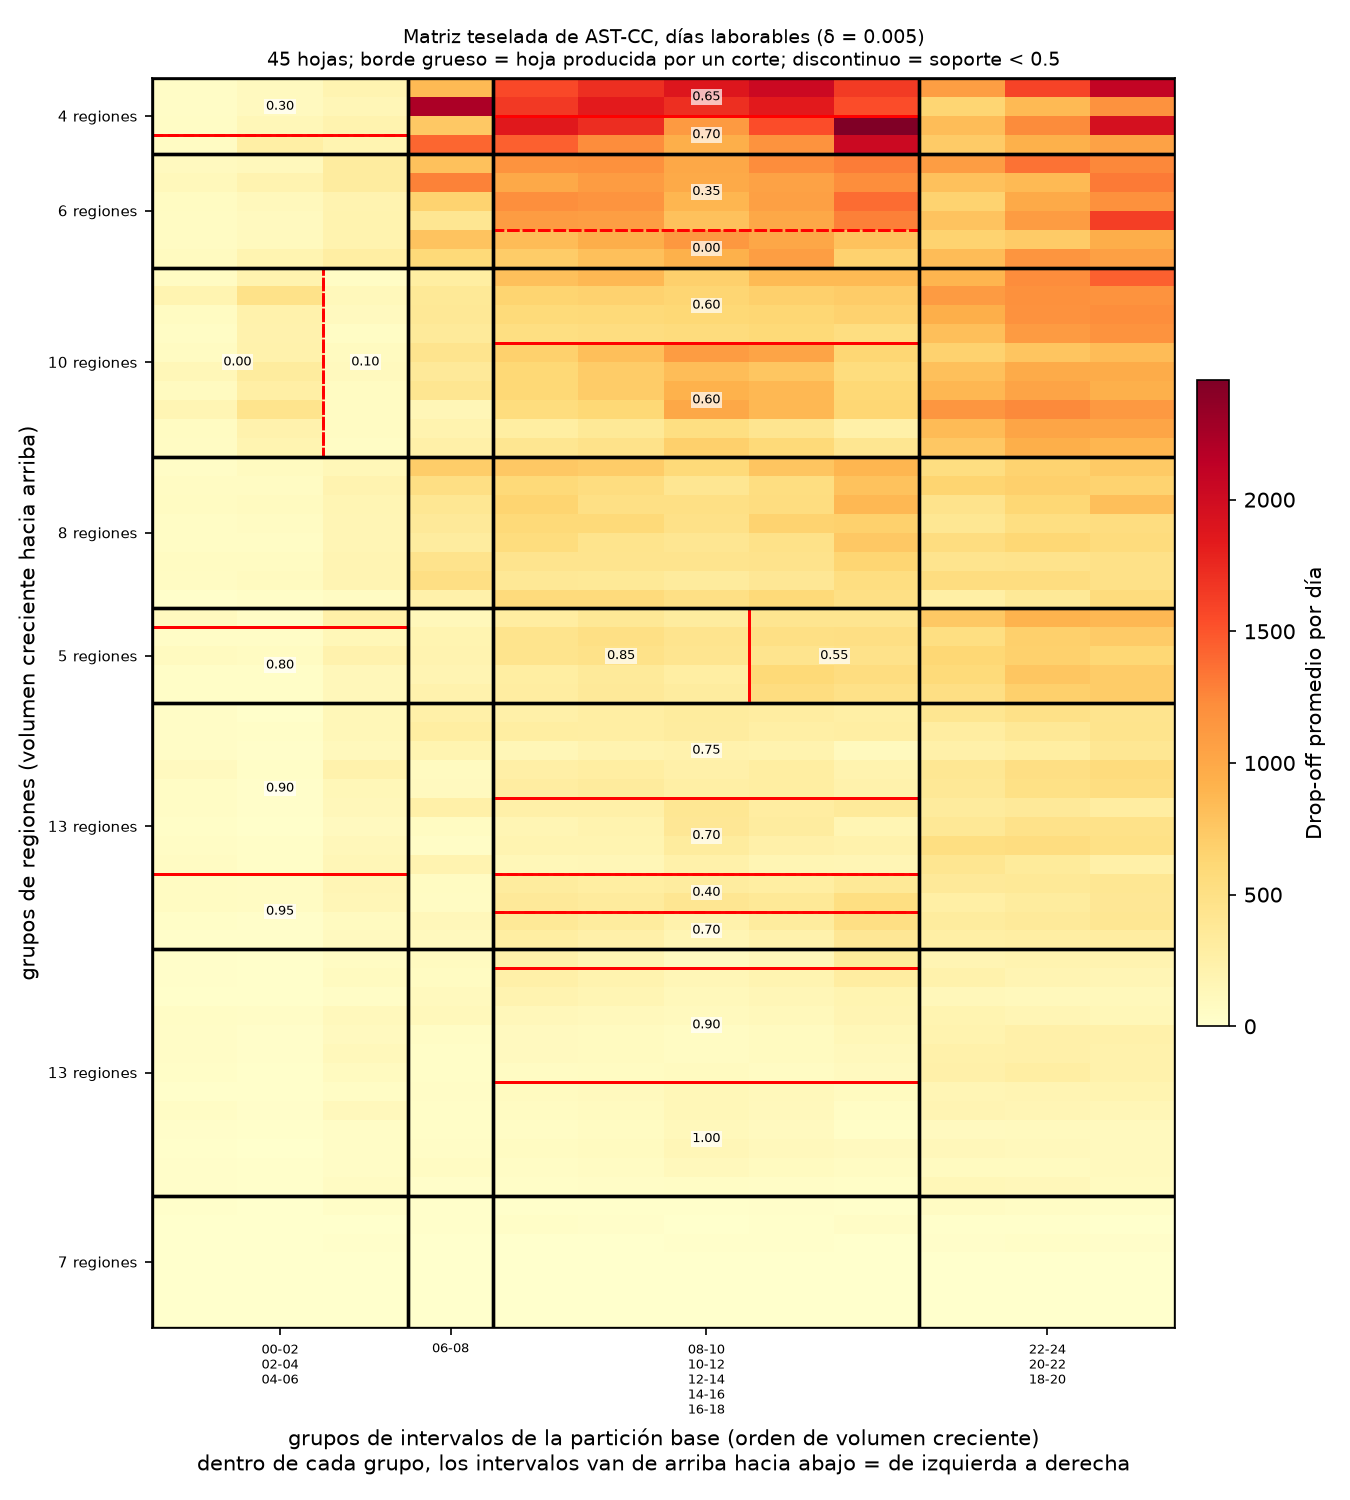
\includegraphics[width=0.85\textwidth]{figs/res/teselada_weekday.png}
\caption{Matriz teselada del árbol resumido del periodo laborable. Los
rectángulos negros son los bloques base de ST-CC, las líneas rojas los cortes de
AST-CC y los números la frecuencia de soporte de cada hoja producida por un corte
(Sección~\ref{sec:res-estabilidad}); el borde discontinuo marca soporte menor que
0.5.}
\label{fig:res-teselada}
\end{figure}

\begin{figure}[t]
\centering
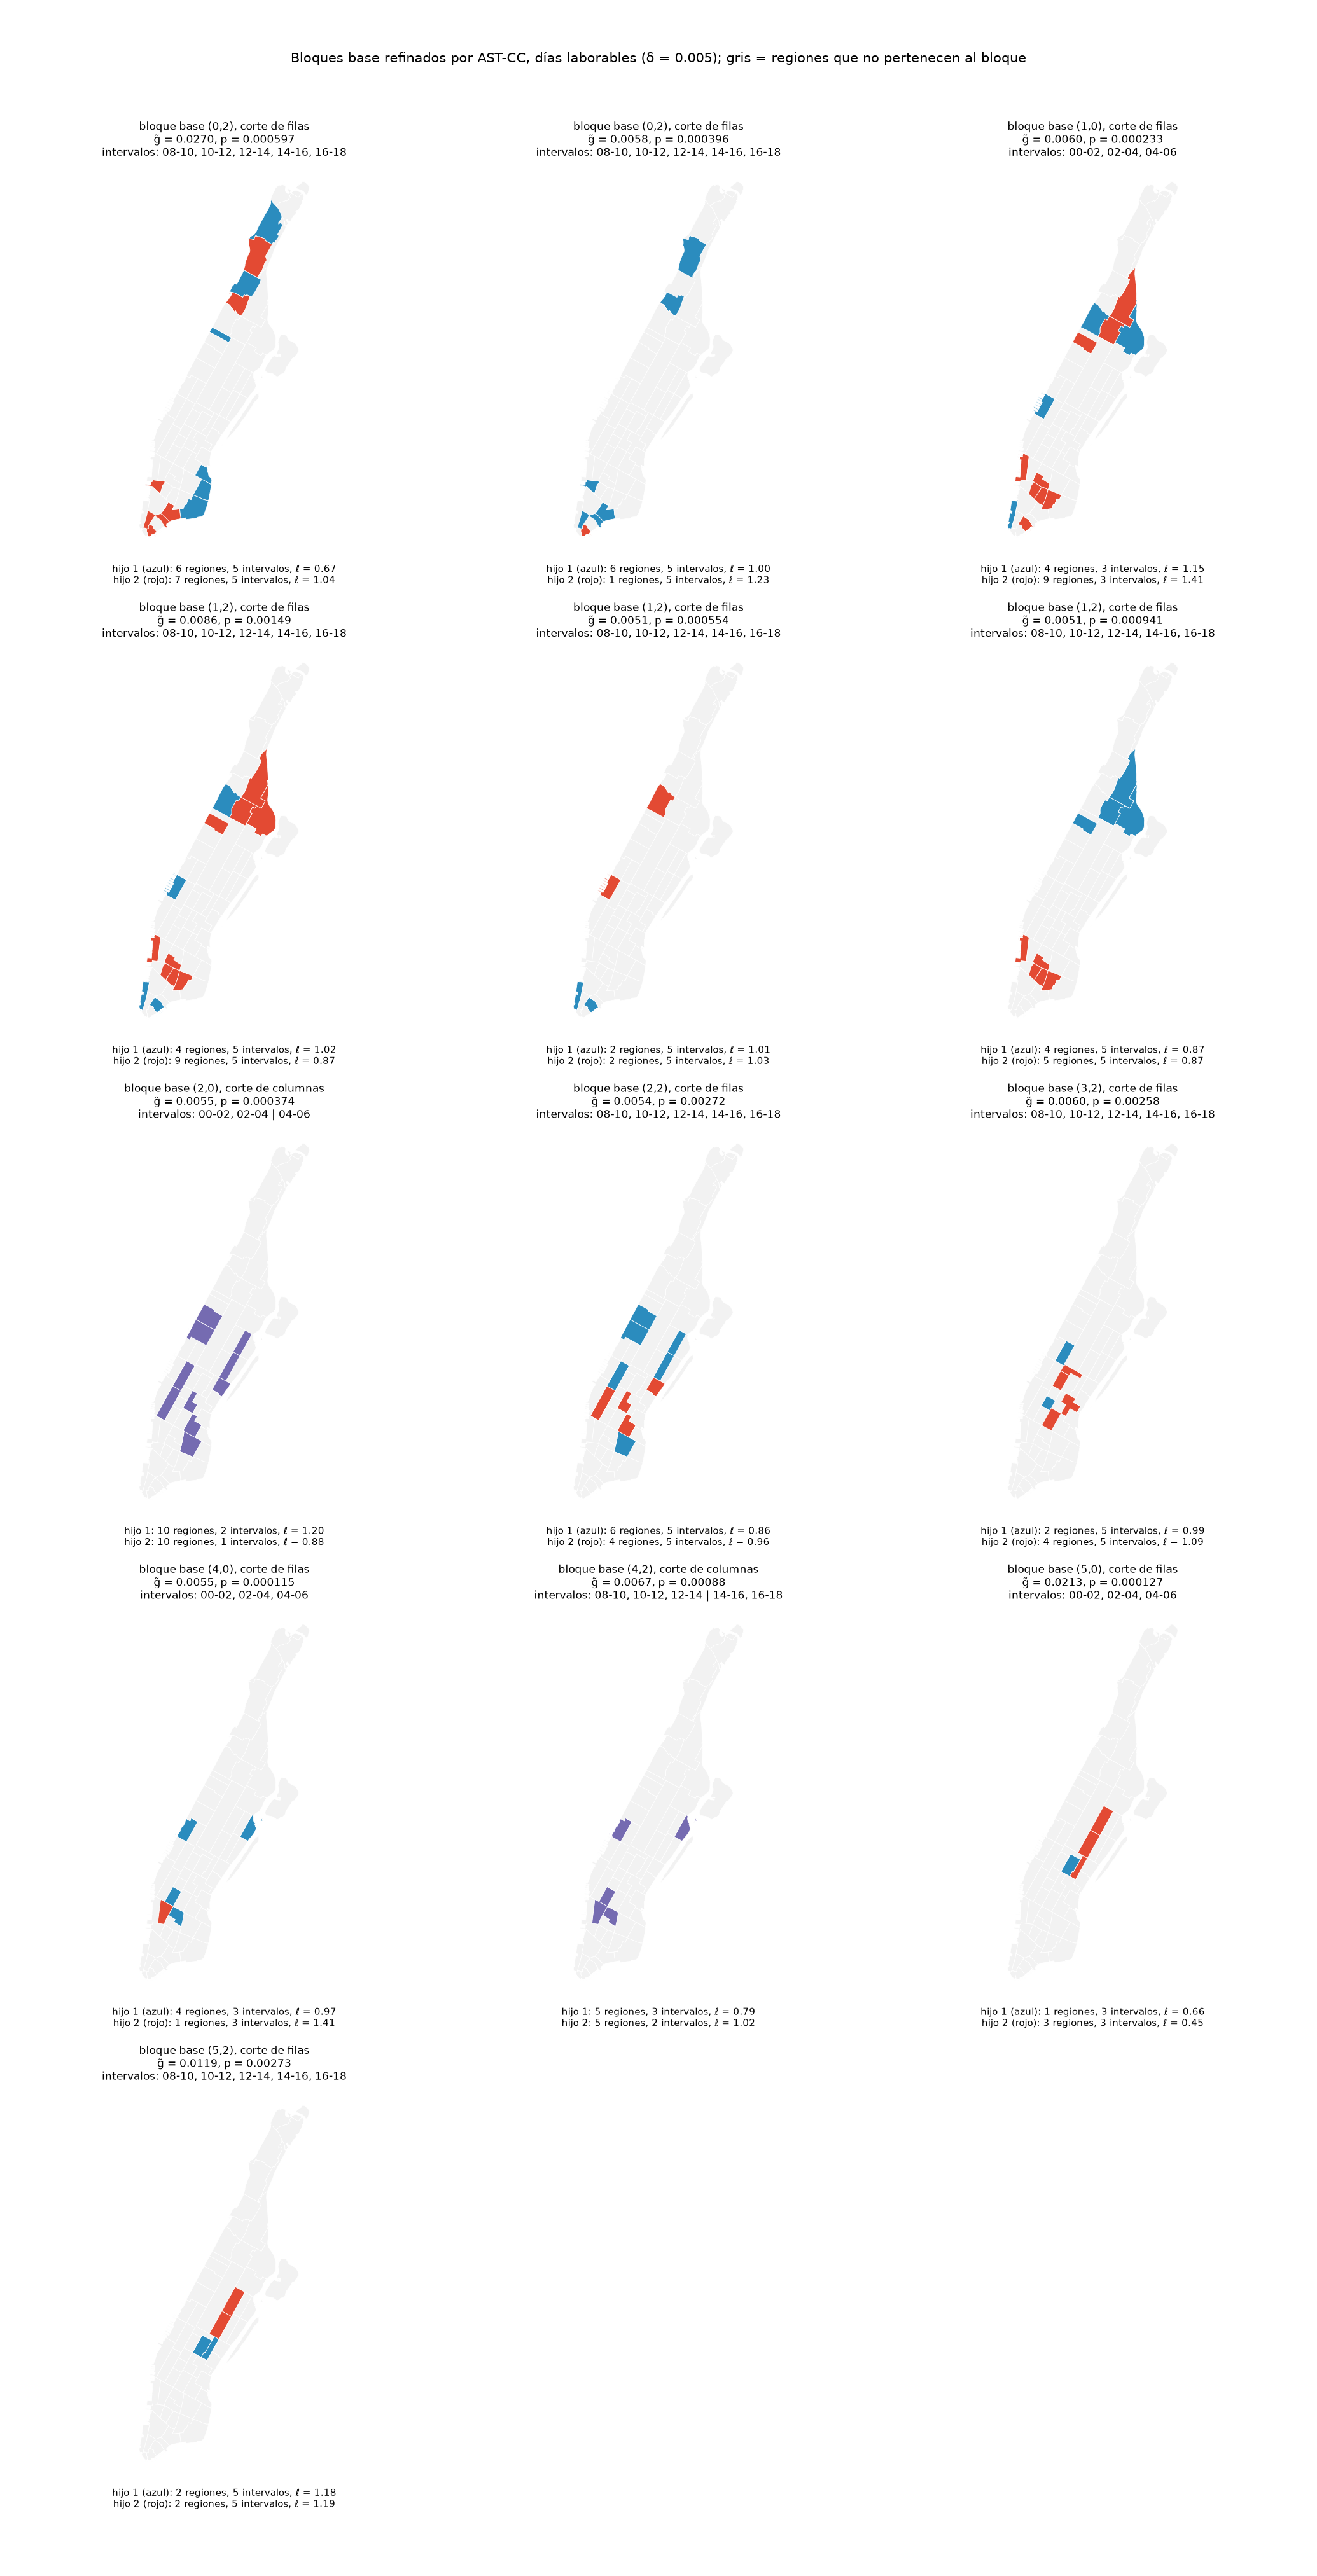
\includegraphics[width=\textwidth]{figs/res/refinados_weekday.png}
\caption{Regiones que separa cada corte del árbol resumido del periodo laborable.
Azul y rojo son los dos hijos de cada corte de filas, y gris las regiones que no
pertenecen al bloque.}
\label{fig:res-refinados}
\end{figure}

Los demás cortes del periodo laborable afectan a la madrugada y a la división de
los intervalos. En el grupo de 00--02 a 04--06, Midtown Center recibe el 52.6\,\%
de sus llegadas nocturnas entre las 4 y las 6, frente al 31.8\,\% de Midtown
East y del Upper East Side, lo que corresponde a la llegada temprana de
trabajadores a una zona de oficinas. Es un patrón claro pero de volumen modesto,
de unas 277 llegadas diarias entre las 4 y las 6 sobre las 526 que recibe Midtown
Center entre la medianoche y las 6. La hoja de Midtown Center reaparece en todas
las ejecuciones con otra partición de partida, mientras que la de Midtown East y
el Upper East Side solo en el 30\,\% de ellas, porque esas regiones cambian de
bloque base entre ejecuciones, de modo que lo estable es que Midtown Center se
separa de su bloque y no el grupo exacto con que se compara. Los dos cortes de
columnas separan, en un bloque, la mañana de 08--14 de la tarde de 14--18, lo que
indica que en ese grupo de regiones la agrupación temporal de ST-CC era demasiado
gruesa, y, en otro, la madrugada profunda de 00--04 del intervalo de 04--06,
aunque este último no reaparece con otras particiones de partida, con soportes de
0 y 0.1, y no se interpreta. La
Figura~\ref{fig:res-refinados} muestra además que los grupos de regiones de ST-CC
están dispersos por toda la isla, porque se forman por volumen, mientras que
varios cortes separan grupos espacialmente compactos, como Midtown frente al Upper
East Side.

\subsection{Árbol resumido del periodo feriado}

En el periodo feriado la partición de ST-CC agrupa los intervalos de una forma
que el árbol pone en evidencia. Como la base C2 junta intervalos de volumen
parecido, ST-CC reúne en un mismo grupo las 02--04 con las 08--10, las 04--06 con
las 06--08, y la medianoche con las 10--12 y la última parte de la noche, aunque
corresponden a momentos del día sin relación entre sí. La mayoría de los cortes
separan precisamente esos intervalos mezclados. En East Village, Clinton East,
Murray Hill y Times Square el 61.0\,\% de las llegadas del grupo 02--04 y 08--10
ocurre de madrugada, frente al 23.7\,\% en Lincoln Square East, Midtown Center,
Penn Station y los Upper East y West Side, donde predominan las llegadas de la
mañana, y en East Village esa fracción llega al 80\,\%. Es la diferencia entre
las zonas de ocio nocturno y las residenciales o de servicios, que en ST-CC
quedaba oculta dentro de un mismo bloque. El corte de mayor ganancia separa, en
el grupo de regiones de menor volumen, Battery Park y Randalls Island, que reciben
el 70\,\% de sus llegadas de ese grupo de intervalos entre las 10 y las 12, de
Inwood, Marble Hill, Roosevelt Island y los parques del norte, que las reciben
sobre todo de noche, con una ganancia corregida de $0.140$ nats por viaje. Ese
bloque reúne solo 3\,026 viajes, y el corte resultó significativo con el menor
p-valor que permiten 20\,000 réplicas, de modo que con un máximo menor no habría
podido probarse, aunque se replica con claridad en el resto de 2017.

Tres advertencias se aplican a la lectura de todos estos cortes. La primera es la
de la Sección~\ref{sec:res-reparacion}, ya que cada corte indica con fundamento que
ST-CC reunió regiones o intervalos con perfiles distintos y dice dónde, pero sus hojas
son la corrección más sencilla que encontró el árbol y no unidades naturales de la
ciudad. La segunda es que el árbol resumido reúne los cortes más fuertes, pero no
es exactamente una poda del árbol completo. Como el conjunto de cortes admisibles
depende de $\delta$, en un mismo bloque el desempate por $z$ puede elegir con el
$\delta$ del resumido un corte distinto del que elige con el del completo, y por
eso 8 de las 105 hojas del árbol completo del periodo laborable y 9 de las 78 del
feriado, que reúnen alrededor del 3\,\% de los viajes, atraviesan una hoja del
resumido. En el resto de la matriz las hojas del árbol completo subdividen las del
resumido, y los cortes de ambos árboles se sostienen fuera de la muestra, como
muestran las Secciones~\ref{sec:res-delta} y \ref{sec:res-estabilidad}. La
tercera es que no todas las hojas del resumido son igual de estables frente a la
partición de partida, y las que reaparecen en menos de la mitad de las ejecuciones
de la Sección~\ref{sec:res-estabilidad} no se interpretan aunque la diferencia
que describen se replique en el resto de 2017. En el periodo feriado, los cortes
descritos en esta sección tienen todos un soporte de al menos 0.95.

% ---------------------------------------------------------------------
\section{Elección de $\delta$ y validación fuera de la muestra}\label{sec:res-delta}

El umbral $\delta$ es el único parámetro de AST-CC que decide cuántos cortes se
aceptan, porque con decenas de miles de viajes por bloque la prueba rechaza casi
siempre y el árbol se detiene por $\delta$ y no por la prueba. El
Capítulo~\ref{chap:propuesta} dejó su valor sin fijar a priori, y la forma natural
de elegirlo es con datos que el árbol no vio. Para ello el árbol se ajustó con
noviembre para cada valor de una rejilla de $\delta$ entre 0.0001 y 0.02, y se
evaluó con tres criterios sobre los otros once meses de 2017. El primero es el
ajuste fuera de la muestra, medido con la divergencia entre la matriz de cada mes
y la predicción de noviembre, dividida por el número de viajes del mes y
promediada sobre los once meses, en milésimas de nat por viaje. El segundo es la
estabilidad, medida con la frecuencia de soporte de las hojas producidas por un
corte en 20 ajustes con el 75\,\% de los días de noviembre elegidos al azar. El
tercero es la replicación, que es la fracción de cortes cuya ganancia, calculada
en el resto de 2017 con los grupos que eligió noviembre, alcanza el mismo $\delta$
con que se aceptó. La Tabla~\ref{tab:res-delta} reúne los tres criterios.

\begin{table}[t]
\centering
\small
\begin{tabular}{@{}lccccccc@{}}
\toprule
$\delta$ & Cortes & $k$ & Pérdida & Soporte & Replicación & $\tilde g$ nov. & $g$ resto \\
\midrule
\multicolumn{8}{@{}l}{Periodo laborable} \\
sin cortes & 0  & 328 & 10.803 & --   & --       & --     & --     \\
0.02     & 2  & 334 & 10.015 & --   & 100\,\% & 0.0241 & 0.0241 \\
0.01     & 3  & 338 & 8.671  & 1.00 & 100\,\% & 0.0201 & 0.0203 \\
0.005    & 13 & 379 & 6.051  & 0.96 & 69\,\%  & 0.0092 & 0.0091 \\
0.0025   & 25 & 420 & 4.990  & 0.94 & 92\,\%  & 0.0063 & 0.0062 \\
0.001    & 49 & 453 & 4.435  & 0.81 & 94\,\%  & 0.0039 & 0.0039 \\
0.0005   & 67 & 496 & 4.009  & 0.77 & 93\,\%  & 0.0031 & 0.0031 \\
0.00025  & 71 & 501 & 3.955  & 0.78 & 96\,\%  & 0.0029 & 0.0029 \\
0.0001   & 72 & 500 & 3.983  & --   & 99\,\%  & 0.0028 & 0.0028 \\
saturado & -- & 792 & 3.767  & --   & --       & --     & --     \\
\midrule
\multicolumn{8}{@{}l}{Periodo feriado} \\
sin cortes & 0  & 312 & 26.674 & --   & --       & --     & --     \\
0.02     & 15 & 364 & 16.708 & --   & 87\,\%  & 0.0379 & 0.0363 \\
0.01     & 24 & 365 & 13.261 & 0.84 & 96\,\%  & 0.0275 & 0.0264 \\
0.005    & 37 & 382 & 11.622 & 0.81 & 84\,\%  & 0.0201 & 0.0191 \\
0.0025   & 42 & 397 & 10.861 & 0.87 & 95\,\%  & 0.0178 & 0.0170 \\
0.001    & 49 & 417 & 10.572 & 0.81 & 96\,\%  & 0.0155 & 0.0146 \\
0.00025  & 52 & 424 & 10.548 & 0.82 & 98\,\%  & 0.0145 & 0.0137 \\
saturado & -- & 792 & 9.113  & --   & --       & --     & --     \\
\bottomrule
\end{tabular}
\caption{AST-CC sobre la partición de ST-CC, ajustado con noviembre de 2017 y
evaluado con los otros once meses. La pérdida es la divergencia fuera de la
muestra en milésimas de nat por viaje, el soporte es el medio de las hojas
producidas por un corte en ajustes con el 75\,\% de los días, la replicación es
la fracción de cortes cuya ganancia en el resto de 2017 alcanza $\delta$, y las
dos últimas columnas son la ganancia media de los cortes en noviembre, corregida
por sesgo, y en el resto del año. En el periodo feriado los valores 0.0001 y
0.0005 producen el mismo árbol que 0.00025.}
\label{tab:res-delta}
\end{table}

El ajuste fuera de la muestra no permite elegir $\delta$. La pérdida baja al
reducir $\delta$, desde 10.80 sin cortes hasta 3.96 con el árbol completo en el
periodo laborable, y el mejor modelo de todos es el saturado, que predice cada mes
con las proporciones de noviembre celda por celda, con 3.77. La diferencia entre
el árbol completo y el saturado, de 0.19, equivale a unos diez errores estándar de
la diferencia pareada entre meses, de modo que la regla de un error estándar, que
elegiría el modelo más sencillo indistinguible del mejor, elige también el
saturado. En el periodo feriado ocurre lo mismo. Esto no indica un defecto del
árbol sino una propiedad de los datos. Con cuarenta millones de viajes en la
evaluación, las proporciones de cada celda se estiman con tanta precisión que
cualquier estructura real, por pequeña que sea, mejora la predicción, y la
validación predictiva solo responde si la estructura existe, no si merece
reportarse.

La estabilidad y la replicación tampoco penalizan los valores pequeños de
$\delta$. En el periodo laborable el soporte de las hojas producidas por un corte
está entre 0.77 y 1 para todos los valores, y en el feriado entre 0.81 y 0.87, de
modo que quitar una cuarta parte de los días no cambia los cortes. La replicación
es de al menos el 92\,\% en el periodo laborable y del 95\,\% en el feriado para
todos los $\delta$ hasta 0.0025, y la ganancia media de los cortes en el resto del
año es prácticamente igual a la de noviembre en toda la rejilla, por ejemplo
0.0029 frente a 0.0029 con el árbol completo del periodo laborable. Si los cortes
de $\delta$ pequeño se ajustaran al ruido de noviembre, su ganancia se encogería
fuera de la muestra, y no lo hace. La replicación más baja, del 69\,\% con
$\delta = 0.005$ en el periodo laborable, se debe a cortes cuya ganancia está muy
cerca del umbral, que en el resto del año quedan apenas por debajo sin que su
ganancia media cambie, con 0.0092 en noviembre y 0.0091 en el resto.

Ninguno de los tres criterios señala, por tanto, un valor de $\delta$ a partir del
cual los cortes dejen de ser reales, y por eso $\delta$ no se trata en esta tesis
como un parámetro estadístico sino como un umbral de resolución, con dos niveles
que cumplen papeles distintos. El árbol completo usa $\delta = 0.00025$, el valor
a partir del cual el árbol deja de cambiar, ya que bajar a 0.0001 solo añade un
corte y no mejora la pérdida, que pasa de 3.955 a 3.983 en el periodo laborable, y
no cambia el árbol en el feriado. Que con 0.0001 el número de parámetros baje en
uno pese a haber un corte más se debe a que los árboles no están anidados, porque
con un $\delta$ menor entran más cortes admisibles y el desempate por $z$ puede
elegir otro en algún bloque. Ese valor tampoco es arbitrario en escala, porque
coincide en orden de magnitud con el umbral que impone el criterio $J$ de la
Sección~\ref{sec:res-comparacion}. Un corte que añade $\Delta k$ parámetros
reduce $J$ solo si su ganancia supera $\log(N)\,\Delta k/(2N_B)$, y en un bloque
de 100\,000 viajes y cinco intervalos, donde un corte de filas añade
$\Delta k = 4$, eso equivale a 0.0003 nats por viaje. Es el modelo que se compara con ST-CC y con las
rejillas en la Sección~\ref{sec:res-comparacion}. El árbol resumido usa el
$\delta$ que deja del orden de 10 a 15 cortes, 0.005 en el periodo laborable y
0.02 en el feriado, porque un árbol de 70 cortes no puede describirse ni
dibujarse, y es el que se interpretó en la Sección~\ref{sec:res-arbol}. El segundo
valor es mayor en el feriado porque los bloques de ST-CC son allí mucho más
heterogéneos, con una ganancia media de los cortes cinco veces mayor que en el
periodo laborable. Ninguna conclusión estadística depende de esa elección, ya que
el árbol resumido reúne los cortes más fuertes y, como los del árbol completo,
estos se sostienen fuera de la muestra, aunque el resumido no sea exactamente una
poda del completo (Sección~\ref{sec:res-arbol}).

% ---------------------------------------------------------------------
\section{Comparación con ST-CC y con rejillas globales}\label{sec:res-comparacion}

Esta sección responde el objetivo de comparar AST-CC con el método base y con la
alternativa más directa, que es una rejilla global más fina. Todos los modelos se
comparan en la misma escala, la de un modelo de Poisson sobre la matriz de
conteos, con la divergencia $D_I(O \,\|\, \hat O)$, el número de parámetros
libres $k$ y el criterio $J = D_I + \tfrac{1}{2}\log(N)\,k$
\eqref{eq:prop-bic}. Como la matriz es una suma de días con más varianza que la
de Poisson, se reporta también $J_\varphi$, que divide la divergencia entre la
dispersión estimada, de 2.06 en el periodo laborable y de 6.73 en el feriado, y que
penaliza más la complejidad. Las rejillas se optimizan directamente para el modelo
de las hojas, de independencia dentro de cada bloque, partiendo de las
particiones de BBAC$_I$ en las bases C2 y C5, lo que las convierte en rivales
exigentes, ya que sin esa optimización su divergencia es entre 1.5 y 4 veces
mayor. Como ni $D_I$ ni $J$ descuentan que la partición y los cortes se eligen con
los mismos datos, la comparación se completa con dos evaluaciones fuera de la
muestra, la de los once meses restantes de 2017 de la
Sección~\ref{sec:res-delta} y una división de los días de noviembre en dos
mitades, en la que cada modelo se ajusta con una mitad y se evalúa con la otra.

\begin{table}[t]
\centering
\small
\begin{tabular}{@{}lrrrr@{}}
\toprule
Modelo & $k$ & $D_I$ & $J$ & $J_\varphi$ \\
\midrule
\multicolumn{5}{@{}l}{Periodo laborable ($N = 3\,602\,851$)} \\
ST-CC, bloques constantes (C2)            & 32  & 161\,319 & 161\,560 & 78\,563 \\
ST-CC, independencia por bloque (C6)      & 328 & 25\,703  & 28\,179  & 14\,955 \\
AST-CC, árbol completo                    & 501 & 1\,045   & 4\,827   & 4\,289 \\
Rejilla $16 \times 6$ ($k$ menor)         & 492 & 1\,954   & 5\,668   & 4\,663 \\
Rejilla $20 \times 6$ ($k$ mayor)         & 516 & 1\,401   & 5\,296   & 4\,575 \\
Rejilla $32 \times 6$ (menor $J$)         & 588 & 574      & 5\,013   & 4\,717 \\
Rejilla $24 \times 4$ (menor $J_\varphi$) & 456 & 2\,085   & 5\,528   & 4\,455 \\
\midrule
\multicolumn{5}{@{}l}{Periodo feriado ($N = 2\,389\,795$)} \\
ST-CC, bloques constantes (C2)            & 24  & 89\,315  & 89\,491  & 13\,457 \\
ST-CC, independencia por bloque (C6)      & 312 & 43\,011  & 45\,302  & 8\,687 \\
AST-CC, árbol completo                    & 424 & 4\,008   & 7\,122   & 3\,710 \\
Rejilla $20 \times 4$ (mismo $k$)         & 424 & 1\,662   & 4\,776   & 3\,361 \\
Rejilla $20 \times 6$ (menor $J$)         & 516 & 864      & 4\,653   & 3\,918 \\
Rejilla $12 \times 2$ (menor $J_\varphi$) & 252 & 5\,943   & 7\,794   & 2\,734 \\
\bottomrule
\end{tabular}
\caption{Ajuste a la matriz de noviembre de 2017. Para cada periodo se muestran
ST-CC en dos modelos, el árbol completo de AST-CC sobre la partición de ST-CC, las
rejillas globales optimizadas con el número de parámetros más cercano por debajo y
por encima del árbol, que en el periodo feriado coinciden en una con el mismo
número, y las rejillas con menor $J$ y menor $J_\varphi$ entre todas las
evaluadas, de $2 \times 2$ a $32 \times 8$.}
\label{tab:res-comparacion}
\end{table}

\subsection{Frente a ST-CC}

La Tabla~\ref{tab:res-comparacion} muestra primero lo que ST-CC deja sin explicar.
En su propio modelo de bloques constantes, ST-CC tiene una divergencia de
161\,319 nats con 32 parámetros en el periodo laborable, y aun permitiendo que cada
bloque tenga sus propios efectos de región y de intervalo, que es el modelo C6 de
328 parámetros, quedan 25\,703 nats de interacción dentro de los bloques. El árbol
completo reduce esa divergencia a 1\,045 nats con 173 parámetros más, es decir,
elimina el 95.9\,\% de lo que ST-CC deja dentro de sus bloques, y en el feriado la
reduce de 43\,011 a 4\,008, el 90.7\,\%. Fuera de la muestra la mejora se
mantiene, ya que la pérdida en los once meses restantes baja de 10.80 a 3.96
milésimas de nat por viaje en el periodo laborable y de 26.67 a 10.55 en el
feriado (Tabla~\ref{tab:res-delta}). En ambos periodos, por tanto, AST-CC mejora
claramente a ST-CC, que es lo que plantea el objetivo general.

\subsection{Frente a rejillas globales}

La comparación con las rejillas da resultados distintos en cada periodo. En el
periodo laborable el árbol completo tiene una divergencia de 1\,045 nats, un
47\,\% menor que la de la mejor rejilla con menos parámetros, la de
$16 \times 6$ con 1\,954, y un 25\,\% menor que la de la rejilla con el número
de parámetros inmediatamente superior, la de $20 \times 6$ con 1\,401. Para
acercarse a su nivel una rejilla necesita al menos 540 parámetros, 39 más que el
árbol, con los que la de $24 \times 6$ queda a un nat, con 1\,046, y la primera
que lo iguala o mejora es la de $12 \times 8$, con 576 parámetros, 75 más. El árbol
tiene además un $J$ menor que el de todas las rejillas evaluadas, con 4\,827
frente a 5\,013 de la mejor, y también un $J_\varphi$ menor, con 4\,289 frente a
4\,455. Fuera de la muestra el árbol completo alcanza la misma pérdida que la
rejilla de $24 \times 6$ con 39 parámetros menos, 3.96 frente a 3.98 en los once
meses restantes, una diferencia comparable al error estándar de la diferencia
pareada entre meses, de unas dos centésimas, y supera con claridad a la rejilla de
$16 \times 6$, con 4.18. En la división de los días de noviembre, en cambio,
la ventaja se reduce a un empate, ya que el árbol gana en el 81\,\% de los 16
ajustes a la rejilla con menos parámetros, pero solo en el 50\,\% a la rejilla con
más, con una diferencia media de 101 nats a favor de esta, dentro de una
desviación típica de 1\,201. Con solo seis días por mitad, la partición base
estimada en cada mitad es más inestable, lo que perjudica más al árbol, que
depende de ella, que a la rejilla. Los árboles ajustados sobre las particiones de
partida más estables de la Sección~\ref{sec:res-sensibilidad} lo confirman, ya
que en la misma división de días ganan a la rejilla con más parámetros en el
94\,\% de los ajustes sobre la base C5 y en el 100\,\% sobre la rejilla optimizada.

En el periodo feriado la rejilla gana. El árbol completo tiene una divergencia
de 4\,008 nats con 424 parámetros, 2.4 veces la de la rejilla de $20 \times 4$
con el mismo número de parámetros, y su $J$ es 2\,469 mayor que el de la mejor
rejilla. Fuera de la muestra el resultado es el mismo, con una pérdida de 10.55
frente a 9.93 de la rejilla de $12 \times 4$, que tiene 64 parámetros menos, y en
la división de días el árbol pierde en todos los ajustes. El árbol mejora mucho a
ST-CC en este periodo, pero no lo suficiente para alcanzar a una rejilla global
optimizada. La razón está en la partición de partida, que en el periodo feriado es
especialmente pobre, con una pérdida fuera de la muestra sin cortes de 26.67,
frente a 10.69 de una rejilla del mismo tamaño optimizada para el modelo de las
hojas. Sus grupos de intervalos reúnen momentos del día sin relación entre sí
(Sección~\ref{sec:res-arbol}), y varios de sus bloques son tan pequeños que el
árbol no puede refinarlos, porque quedan por debajo de $N_{\min}$ o porque su
nivel $\alpha_B$ no alcanza a resolverse con las réplicas disponibles. La
sección siguiente muestra que, con una partición de partida mejor, el árbol sí
compite con las rejillas en ese periodo.

\subsection{Sensibilidad a la partición base}\label{sec:res-sensibilidad}

Para separar el efecto del árbol del de la partición de partida, AST-CC se ajustó
también sobre la partición de BBAC$_I$ en la base C5 y sobre la rejilla de
$K_R \times K_T$ optimizada para el modelo de las hojas, que es la mejor partición
de ese tamaño para este modelo. Ninguna de las dos se parece a la de ST-CC, con
índices de Rand ajustados en las filas de 0.08 y 0.09 en el periodo laborable. En
ese periodo los tres árboles completos llegan al mismo lugar, con divergencias de
1\,045, 989 y 901 nats y entre 470 y 501 parámetros, pérdidas fuera de la muestra
de 3.96, 3.97 y 3.97, y valores de $J$ de 4\,827, 4\,657 y 4\,449, todos menores
que el de la mejor rejilla. El resultado del periodo laborable no depende, por
tanto, de la partición de partida. Sobre esas dos bases el árbol completo sigue
haciendo 77 y 64 cortes, mientras que sobre una partición correcta de datos
sintéticos no hace ninguno (Sección~\ref{sec:res-reparacion}), de modo que en los
días laborables de Manhattan hay interacción local que ninguna rejilla de
$8 \times 4$ captura, y no solo los defectos de una partición que agrupa por
volumen. En el feriado sí depende. Sobre la rejilla
optimizada, el árbol completo tiene una divergencia de 2\,704 nats con 376
parámetros, un 5\,\% menor que la de la rejilla de $24 \times 2$, con 2\,854 y 372,
y sobre la partición de la base C5 alcanza una pérdida fuera de la muestra de 9.66
con 372 parámetros, igual a la de la rejilla de $8 \times 6$, que tiene 72
parámetros más. Con una partición de partida razonable el árbol empata con las
rejillas en el periodo feriado, y la desventaja de la
Tabla~\ref{tab:res-comparacion} se debe a la partición de ST-CC más que al
refinamiento.

% ---------------------------------------------------------------------
\section{Estabilidad y replicación de los cortes}\label{sec:res-estabilidad}

Que un corte sea significativo y supere $\delta$ no garantiza que pueda
interpretarse, porque podría depender de detalles del ajuste que no tienen que ver
con la movilidad. Esta sección somete los cortes del árbol resumido a dos
comprobaciones de distinto tipo. La primera mide cuánto dependen de la partición
de partida, que es la parte más inestable del procedimiento, y la segunda si las
diferencias que describen se mantienen en meses que el árbol no vio. La
estabilidad frente a la muestra de días, con la partición fija, ya se mostró en la
Tabla~\ref{tab:res-delta}, con soportes entre 0.77 y 1 en el periodo laborable y
entre 0.81 y 0.87 en el feriado.

\subsection{Estabilidad frente a la partición de partida}

ST-CC obtiene su partición con BBAC$_I$, que depende de la inicialización y tiene
muchos óptimos locales, de modo que otra ejecución del mismo método puede producir
una partición algo distinta. Para medir cuánto afecta eso a los cortes, el
procedimiento completo se repitió 20 veces con la partición de una sola
inicialización de BBAC$_I$ en la base C2, que es el esquema de ST-CC, y se midió
la frecuencia de soporte de cada hoja del árbol resumido, es decir, la proporción
de ejecuciones en las que aparece una hoja con un índice de Jaccard de al menos
0.5 sobre las celdas. Estas particiones se parecen a la de ST-CC, con índices de
Rand ajustados de 0.79 en las filas y 0.85 en las columnas en el periodo
laborable y de 0.78 y 0.97 en el feriado, pero no son iguales, y solo el 15\,\% de
ellas alcanza o mejora la función objetivo de ST-CC en el periodo laborable, frente
al 75\,\% en el feriado. Aun así, el 74\,\% de las hojas producidas por un corte
tienen un soporte de al menos 0.5 en ambos periodos, con medias de 0.63 en el
periodo laborable y 0.72 en el feriado. Los bloques base sin cortes tienen un
soporte mayor, de 0.78 y 0.92, como es de esperar, porque una hoja producida por un
corte solo reaparece si reaparecen tanto su bloque base como el corte. La
Figura~\ref{fig:res-teselada} indica el soporte de cada hoja, con borde discontinuo
en las seis del periodo laborable que no llegan a 0.5, que no deben interpretarse
como hallazgos aunque superen la prueba y el umbral. Son las del corte que separa
Lincoln Square East y Penn Station de Midtown North, Murray Hill, Times Square y
Union Square, con 0 y 0.35, las del corte de columnas que separa 00--04 de
04--06, con 0 y 0.1, la de Midtown East y el Upper East Side en la madrugada, con
0.3, cuya hermana de Midtown Center tiene soporte 1, y la de Clinton West y
Morningside Heights en el grupo diurno, con 0.4. En el periodo feriado no llegan a
0.5 siete hojas, todas en bloques que reúnen los intervalos que ST-CC mezcló,
04--06 con 06--08 o 02--04 con 08--10, en los grupos de regiones R3 y R4, de
volumen intermedio, mientras que las de los cortes que se interpretan en la
Sección~\ref{sec:res-arbol} tienen un soporte de al menos 0.95. Una hoja con soporte
bajo no indica que la diferencia que describe sea ruido, ya que los 23 cortes de
filas de la Tabla~\ref{tab:res-replicacion}, incluidos los de hojas con soporte
bajo, conservan el orden de sus grupos en el resto de 2017, sino que el árbol solo
llega a ese corte con la partición particular de ST-CC.

\subsection{Replicación en el resto de 2017}

Para cada corte del árbol resumido se calcularon, con los días de noviembre y con
los de los otros once meses de 2017, la cuota de llegadas de cada grupo en cada
intervalo del bloque y la información mutua de la tabla colapsada, que con los
datos de noviembre es la ganancia del corte. Los grupos son los que eligió el
árbol con noviembre, sin volver a ajustarlo. La Tabla~\ref{tab:res-replicacion}
muestra, para cada corte de filas, el intervalo en que los dos grupos más
difieren. En los 23 cortes de filas el grupo con mayor cuota en noviembre la tiene
también en el resto del año, y las diferencias entre grupos, de entre 6.9 y 57.5
puntos porcentuales en noviembre, quedan entre 5.8 y 56.4 en el resto del año. En
el periodo laborable las cuotas de la tabla cambian a lo sumo unos 2 puntos, y
la información mutua del resto del año está entre el 72 y el 114\,\% de la de
noviembre, lo que significa que estos cortes describen rasgos estables de la
movilidad de los días laborables y no particularidades del mes.

En el periodo feriado los cambios son mayores, con cuotas que varían hasta 12.4
puntos, aunque sin invertir nunca el orden de los grupos. La mayor diferencia
aparece en el corte que separa Bloomingdale, el Financial District South y
Washington Heights South de las otras diez regiones de su grupo en el bloque de
04--08, cuyos grupos más difieren en el intervalo de 04--06 y cuya información mutua cae a un tercio fuera de noviembre, de 0.022 a
0.0075 nats por viaje, aunque el grupo sigue recibiendo una fracción menor de sus
llegadas de madrugada que el resto. Solo otro corte queda por debajo del
70\,\%, el del bloque R1-T4, que conserva el 69.9\,\% de su información mutua.
Estos cambios mayores son esperables, ya que los fines de semana
del resto del año abarcan estaciones y temporadas de ocio distintas, y el
periodo feriado de noviembre incluye además el Día de Acción de Gracias. Los
cinco cortes de columnas, que no admiten la misma tabla porque separan
intervalos y no grupos de regiones, conservan entre el 80 y el 110\,\% de su
información mutua en el resto del año.

\begin{table}[t]
\centering
\small
\begin{tabular}{@{}llccccrr@{}}
\toprule
 & & & & \multicolumn{2}{c}{Cuota en el intervalo (\%)} & \multicolumn{2}{c}{$I$ ($10^{-3}$ nats por viaje)} \\
\cmidrule(lr){5-6}\cmidrule(l){7-8}
Periodo & Bloque & Intervalo & Regiones & Noviembre & Resto de 2017 & Nov. & Resto \\
\midrule
Laborable & R2-T3 & 16--18 & 6 / 7 & 29.2 / 13.8 & 28.9 / 13.6 & 27.2 & 26.6 \\
Laborable & R2-T3 & 08--10 & 1 / 6 & 35.3 / 26.4 & 36.0 / 26.3 & 6.0 & 5.5 \\
Laborable & R3-T1 & 04--06 & 4 / 9 & 21.2 / 12.4 & 19.8 / 12.1 & 6.3 & 5.2 \\
Laborable & R3-T3 & 08--10 & 4 / 9 & 27.0 / 17.7 & 27.7 / 17.8 & 8.7 & 9.9 \\
Laborable & R3-T3 & 16--18 & 2 / 2 & 20.0 / 12.9 & 18.5 / 12.7 & 5.2 & 4.8 \\
Laborable & R3-T3 & 16--18 & 4 / 5 & 27.9 / 21.1 & 27.0 / 20.9 & 5.1 & 4.6 \\
Laborable & R6-T3 & 16--18 & 6 / 4 & 25.8 / 18.8 & 25.4 / 18.8 & 5.5 & 5.3 \\
Laborable & R7-T3 & 08--10 & 4 / 2 & 23.4 / 16.2 & 24.1 / 16.2 & 6.0 & 6.7 \\
Laborable & R4-T1 & 04--06 & 4 / 1 & 18.8 / 10.4 & 17.3 / 10.3 & 5.7 & 4.1 \\
Laborable & R8-T1 & 04--06 & 1 / 3 & 52.6 / 31.8 & 50.7 / 29.8 & 21.4 & 21.6 \\
Laborable & R8-T3 & 08--10 & 2 / 2 & 28.9 / 18.3 & 29.9 / 17.9 & 12.0 & 12.8 \\
Feriado & R3-T2 & 02--04 & 9 / 6 & 54.8 / 31.5 & 59.9 / 38.6 & 26.6 & 21.5 \\
Feriado & R3-T2 & 02--04 & 5 / 1 & 36.1 / 11.7 & 42.6 / 17.4 & 24.1 & 20.0 \\
Feriado & R4-T1 & 04--06 & 5 / 5 & 60.2 / 34.7 & 63.1 / 39.9 & 30.6 & 26.0 \\
Feriado & R4-T2 & 02--04 & 7 / 3 & 62.1 / 34.2 & 66.6 / 38.3 & 34.5 & 34.6 \\
Feriado & R2-T1 & 04--06 & 10 / 3 & 64.6 / 42.9 & 68.5 / 55.2 & 22.0 & 7.5 \\
Feriado & R1-T4 & 12--14 & 3 / 4 & 44.0 / 20.1 & 36.8 / 19.4 & 46.9 & 32.8 \\
Feriado & R1-T3 & 10--12 & 2 / 5 & 70.0 / 12.5 & 67.7 / 11.3 & 143.4 & 148.8 \\
Feriado & R6-T1 & 04--06 & 4 / 6 & 51.9 / 29.1 & 58.2 / 32.7 & 26.9 & 32.8 \\
Feriado & R6-T2 & 02--04 & 4 / 6 & 61.0 / 23.7 & 66.8 / 28.6 & 72.2 & 74.5 \\
Feriado & R6-T2 & 02--04 & 1 / 3 & 80.0 / 52.9 & 82.4 / 59.5 & 34.4 & 27.3 \\
Feriado & R6-T3 & 10--12 & 5 / 5 & 37.7 / 20.5 & 37.9 / 19.9 & 24.8 & 25.3 \\
Feriado & R5-T2 & 02--04 & 5 / 6 & 59.3 / 37.3 & 65.3 / 44.0 & 24.3 & 22.9 \\
\bottomrule
\end{tabular}

\caption{Cortes de filas del árbol resumido y su repetición en el resto de 2017.
Cada bloque se identifica por su grupo de regiones R y de intervalos T de
ST-CC, numerados por volumen medio creciente. Para cada corte se muestra el
intervalo en que más difieren los dos grupos, el número de regiones de cada grupo
y su cuota de llegadas en ese intervalo, en noviembre y en el resto del año, y la
información mutua de la tabla colapsada en milésimas de nat por viaje.}
\label{tab:res-replicacion}
\end{table}

% ---------------------------------------------------------------------
\section{Interpretación de los patrones}\label{sec:res-interpretacion}

ST-CC termina asignando a cada bloque un estado de actividad, de muy bajo a alto,
mediante un K-means sobre la media y la desviación típica de sus celdas, y presenta
el resultado como un mapa de estados que puede reunir bloques no contiguos
(Sección~\ref{sec:stcc}). Para ver qué cambia ese mapa al refinar, se aplicó el
mismo procedimiento a las 45 hojas del árbol resumido del periodo laborable y a
las 39 del feriado, con $K = 4$ como \citet{Liu2021}, aunque el índice de silueta
\citep{Rousseeuw1987} favorecería $K = 3$ en ambos periodos, con 0.62 y 0.57 frente a 0.51 y 0.56. La
Figura~\ref{fig:res-antes-despues} compara el mapa de estados de la partición de
ST-CC con el de las hojas, usando los mismos centroides para ambos.

\begin{figure}[t]
\centering
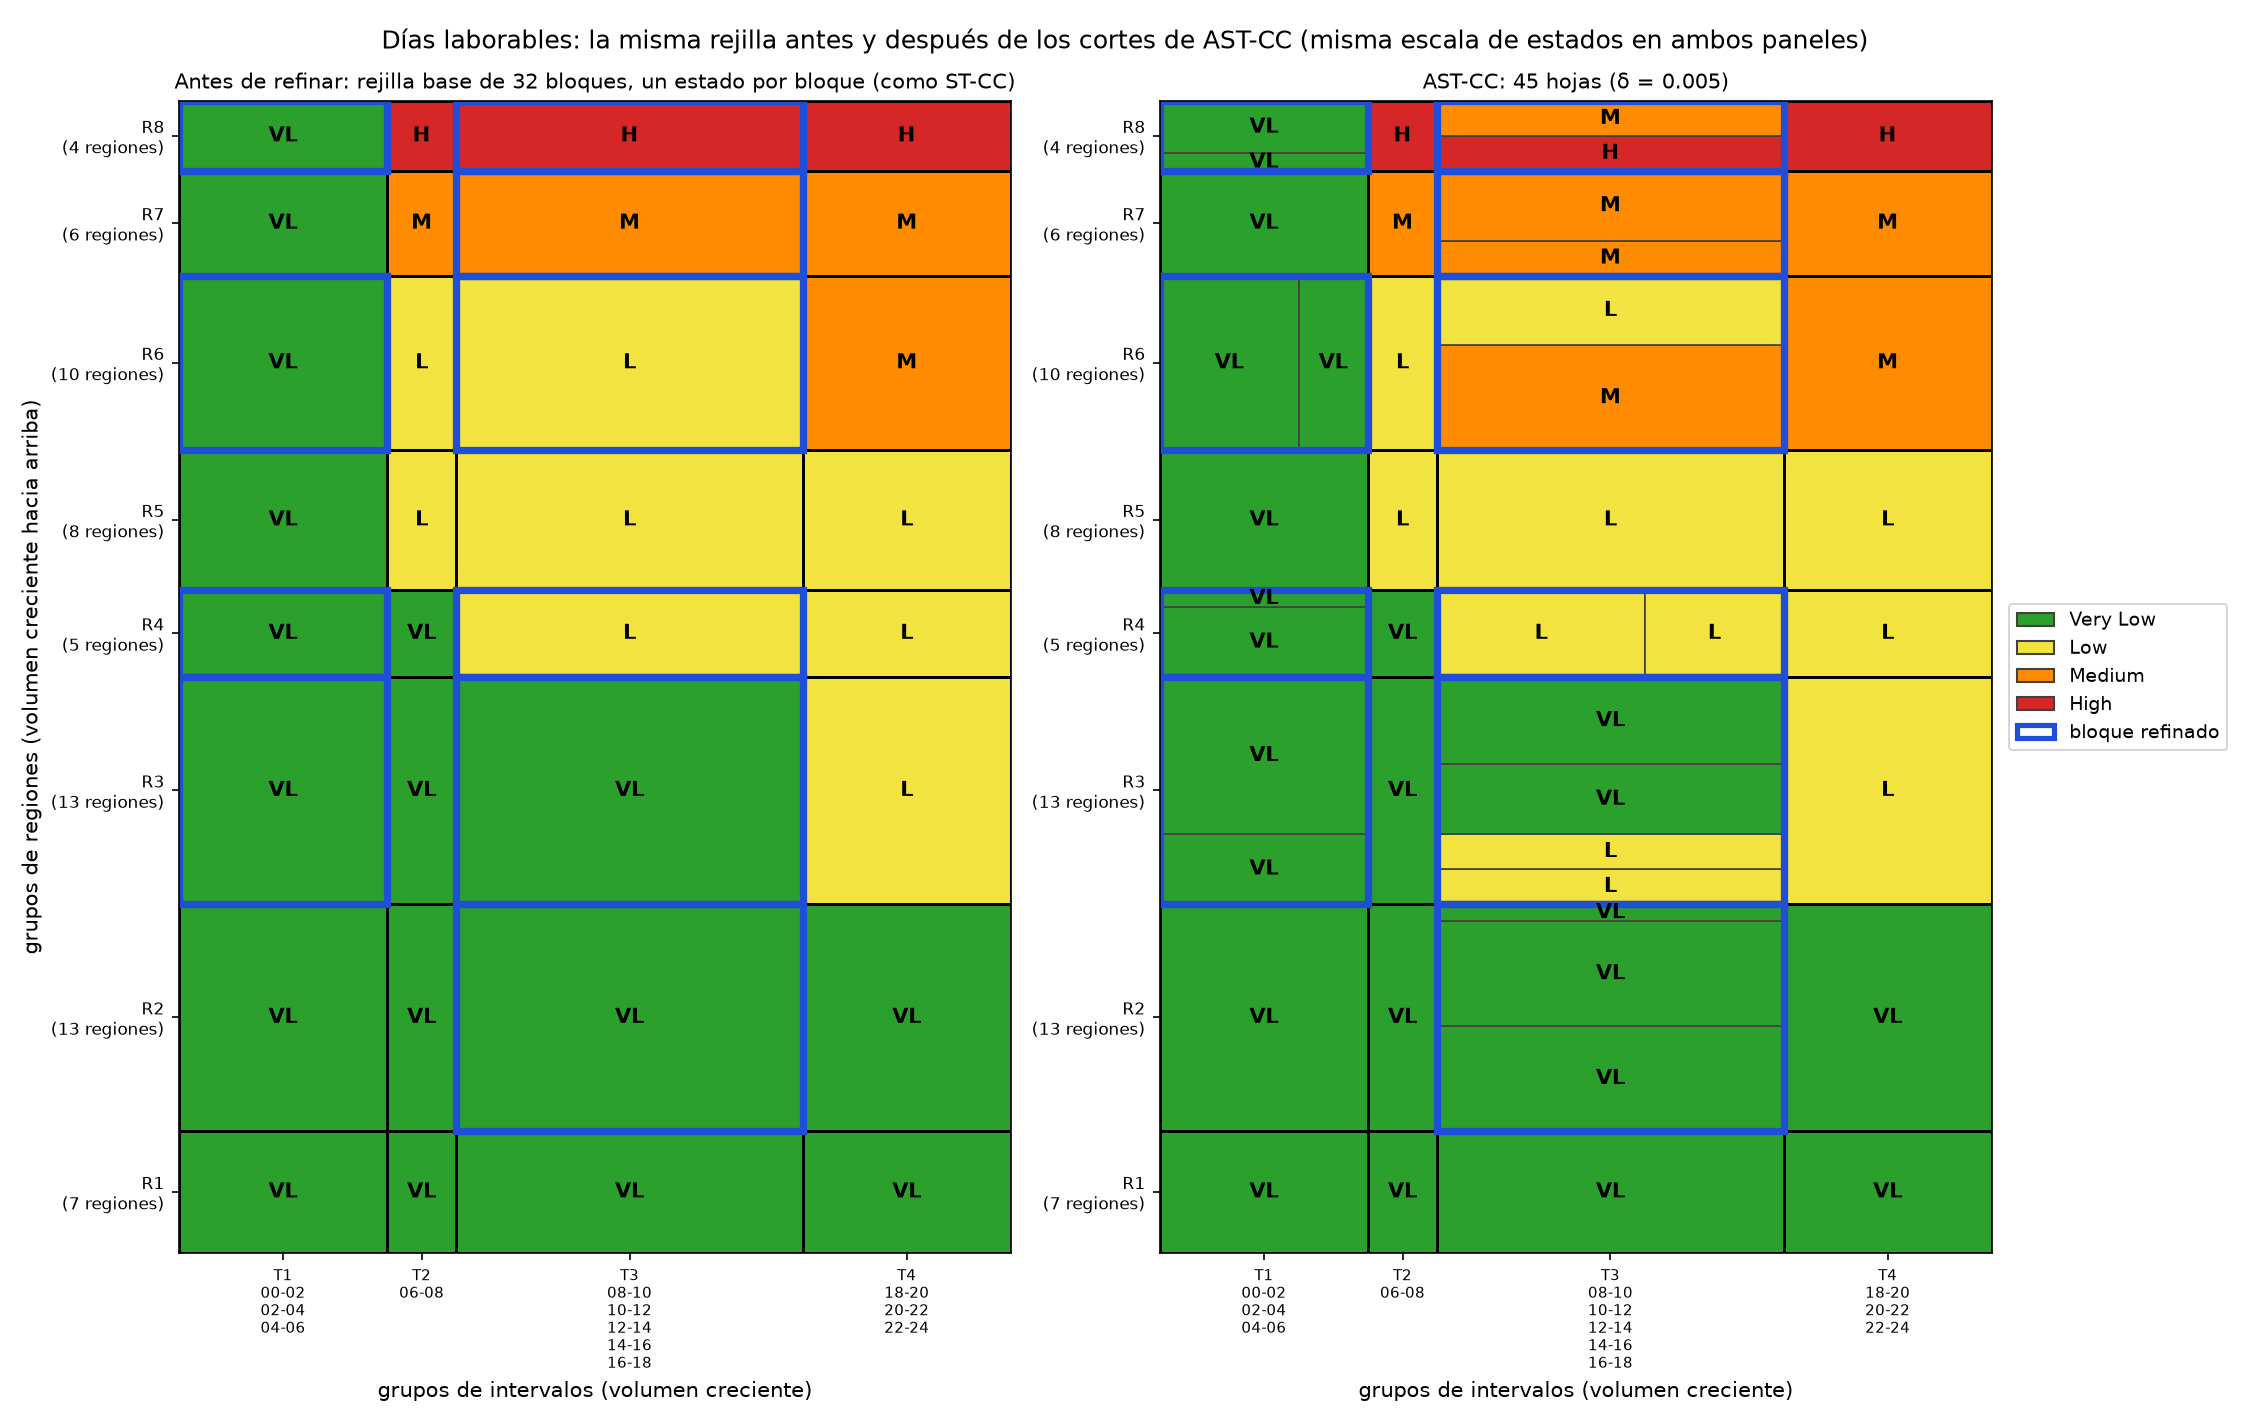
\includegraphics[width=\textwidth]{figs/res/antes_despues_weekday.png}
\caption{Estados de actividad de la partición de ST-CC (izquierda) y de las hojas
del árbol resumido (derecha) en el periodo laborable. Cada bloque base recibe el
estado del centroide más cercano del K-means de las hojas, de modo que los bloques
sin cortes conservan su color.}
\label{fig:res-antes-despues}
\end{figure}

El mapa de estados apenas cambia. De los 10 bloques base que el árbol refina en el
periodo laborable, solo 3 contienen hojas de estados distintos, y en el feriado
solo 4 de 12. La razón es la misma que explica los cortes. La partición de ST-CC
reúne regiones e intervalos de volumen parecido, el árbol los separa por la forma
de su perfil, y la media y la desviación típica de las celdas, que son los
atributos del K-means, miden sobre todo el volumen. Los dos grupos que separa un
corte suelen tener, por tanto, el mismo estado aunque reciban sus viajes a horas
distintas. Cuando el estado cambia, además, no siempre lo hace en la dirección que
sugiere el volumen. Midtown Center y Midtown East quedan en el estado alto con
1\,550 llegadas por celda y día, y el Upper East Side en el medio con 1\,741,
porque el K-means pondera también la desviación típica entre intervalos, que es
mayor en las zonas que se llenan de golpe por la mañana. Lo mismo ocurre en el
bloque R6-T3, donde la hoja de Clinton East, East Village, Lenox Hill West,
Yorkville West y los Upper West Side, con 651 llegadas por celda y día, queda en el
estado medio, y la de East Chelsea, Gramercy, Midtown South y Sutton Place, con
663, en el bajo.

El mapa de estados de ST-CC no es, por tanto, la forma adecuada de leer lo que
encuentra AST-CC, y los patrones deben describirse por el reparto de las llegadas
de cada hoja entre los intervalos de su bloque, como en las
Secciones~\ref{sec:res-arbol} y \ref{sec:res-estabilidad}. Leídos así, los
cortes del árbol resumido revelan tres patrones espacio-temporales locales que
ST-CC no muestra. El primero es el desfase horario del desplazamiento laboral,
en el que, dentro de grupos de zonas con el mismo volumen diario, unas reciben sus
viajes entre las 8 y las 10 y otras entre las 16 y las 18. El segundo es la
llegada temprana a las zonas de oficinas, visible en la madrugada de Midtown
Center, que recibe la mitad de sus llegadas nocturnas entre las 4 y las 6 y cuya
separación reaparece con cualquier partición de partida, aunque el grupo con que
se compara cambie entre ejecuciones. El
tercero, en el periodo feriado, es la separación entre las zonas de ocio nocturno
y las residenciales o de servicios, que ST-CC ocultaba al reunir intervalos de
madrugada y de mañana en un mismo grupo. Los tres son diferencias de horario
entre zonas de volumen parecido, que es exactamente lo que una partición por
volumen no puede ver y lo que el árbol está diseñado para localizar. Todos ellos
se replican en el resto de 2017 (Sección~\ref{sec:res-estabilidad}). Las
etiquetas de oficinas, residencias u ocio se deducen de los nombres y de la
ubicación de las zonas, y no se contrastaron con datos de uso del suelo.

% ---------------------------------------------------------------------
\section{Limitaciones}\label{sec:res-limitaciones}

Los resultados anteriores tienen varias limitaciones que conviene hacer
explícitas. La primera es que en el periodo feriado AST-CC sobre la partición de
ST-CC no alcanza a una rejilla global optimizada, ni en la muestra ni fuera de
ella. La Sección~\ref{sec:res-sensibilidad} atribuye esa desventaja a la partición
de partida, porque con una mejor el árbol empata con las rejillas, pero eso
significa que la mejora que aporta el árbol depende de la calidad de la partición
que refina, y que con una partición tan pobre como la de ST-CC en el feriado el
refinamiento local no basta. Relacionada con ella está la segunda, que en la
división de los días de noviembre en dos mitades el árbol solo empata con las
rejillas en el periodo laborable, de modo que su ventaja requiere días suficientes
para estimar de forma estable la partición de partida.

La tercera limitación es que hay bloques que el método no puede probar. Los
bloques del grupo de regiones de menor volumen tienen tan pocos viajes que su
nivel $\alpha_B$, repartido por masa, queda por debajo de lo que pueden resolver
20\,000 réplicas, y quedan como hojas inalcanzables, cuatro en el árbol completo
del periodo laborable y siete en el feriado. Aumentar el número máximo de
réplicas o agrupar esos bloques antes de probarlos lo resolvería a cambio de
más cómputo o de un reparto de $\alpha$ distinto. El mismo límite afecta a bloques
que sí se prueban, ya que el corte de mayor ganancia del periodo feriado resultó
significativo con el menor p-valor que permiten esas réplicas. La cuarta es que la garantía de
control de error de la Sección~\ref{sec:prop-multiplicidad} es aproximada, porque
la jerarquía se construye con los mismos datos que se prueban, y su validez se
comprobó solo de forma empírica, con datos sintéticos en los que el FWER no superó
0.03. Esa comprobación usó una partición base que recupera los bloques
verdaderos, y la calibración en los bloques nocturnos del periodo feriado sigue
siendo algo liberal, como ya se indicó en el Capítulo~\ref{chap:propuesta}. Esa
liberalidad coincide con que la variabilidad entre días del feriado, con un
cociente mediano de 17.1 entre la varianza y la media, queda por encima de la del
escenario sintético fuerte, de modo que ese régimen no quedó cubierto por la
simulación. Además, los diseños sintéticos favorecen la estructura local,
porque todos los patrones viven en un solo bloque y ocupan la mitad de sus filas y
de sus columnas, lo que se presta a un corte de filas, y ninguno tiene como verdad
una rejilla global más fina, que es el caso en el que la rejilla debería ganar. Si
la estructura de los datos reales es local o global se juzgó con las comparaciones
de la Sección~\ref{sec:res-comparacion}.

La quinta limitación se refiere a la lectura de las hojas. La
Sección~\ref{sec:res-reparacion} mostró que, cuando la partición de partida agrupa
mal, el árbol reconstruye la distribución verdadera, pero con hojas que no
coinciden con los bloques verdaderos, con una pureza de 0.59. Los cortes indican
con fundamento dónde ST-CC mezcló perfiles distintos, pero las hojas no deben
interpretarse como unidades naturales de la ciudad. Por la misma razón, la
fracción del término (iii) que explica el árbol sobre la partición de ST-CC no
mide por sí sola la estructura local, porque sobre una partición que agrupa por
volumen el árbol repara casi todo, y esa evidencia la dan la sensibilidad a la
partición de partida y las comparaciones con las rejillas. Además, una cuarta parte de
las hojas producidas por un corte en el árbol resumido reaparece en menos de la
mitad de las ejecuciones con otra partición de partida, y esas hojas no se
interpretaron aunque las diferencias que describen se repliquen. La sexta es que
$\delta$ no pudo fijarse con datos. Los dos niveles que se usan responden a papeles
distintos y ninguna conclusión estadística depende de ellos, pero el tamaño del
árbol resumido es una elección de presentación, y como el desempate elige entre
cortes admisibles cuyo conjunto depende de $\delta$, los árboles de distintos
$\delta$ no están anidados, de modo que el resumido difiere del completo en cerca
del 3\,\% de los viajes. La séptima es que los p-valores se
obtienen por simulación, de modo que unos pocos cortes cercanos al umbral cambian
con la semilla aleatoria, del orden de dos o tres cortes sobre setenta en el
árbol completo. En el periodo feriado esos pocos cortes pesan más, y con otra
semilla la divergencia del árbol completo pasa de 4\,008 a 3\,486 nats, un 13\,\%
menos, sin que cambie ninguna de las comparaciones con ST-CC ni con las rejillas.
Todos los resultados se reportan con una semilla fija para que sean
reproducibles, y la que se usa no es la más favorable al árbol en el feriado.

Por último, el árbol se ajustó con un solo mes, noviembre de 2017, que es el del
caso de estudio de ST-CC, y aunque sus cortes se replican en el resto del año, no
se comprobó si un árbol ajustado con otro mes encontraría los mismos. Las
interpretaciones de las zonas como de oficinas, residenciales o de ocio se basan en
sus nombres y en las cuotas por intervalo, sin contrastarse con datos externos de
uso del suelo o de empleo, y la coherencia espacial de los grupos que separan los
cortes se observó en los mapas, pero no se cuantificó. Los datos, por último, son
los de \citet{Liu2021} y heredan su alcance, ya que describen solo los viajes en
taxi, cuyos usuarios no representan a toda la población, solo sus destinos y no
los pares de origen y destino, solo Manhattan e intervalos fijos de dos horas.
